
\chapter{Enhancing human-robot physical collaboration with polytopes}
\label{ch:physical_interaction}

\Cref{ch:phisical_ability_metrics} presentes the benefits of polytope representations of physical abilities for robots and humans, based on their musculoskeletal models. Polytopes, in addition to being their accurate representation, can actually be used as a unifying view on their different physical abilities and allow for characterising their common physical abilities, as one system, in the same polytope form. \Cref{ch:transformin_polytopes} then presents some of the most efficient algorithms, proposed in the literature, for transforming different polytope families into the standard forms suitable for different applications, such as visualisation or robot control. Furthermore, in \Cref{ch:transformin_polytopes}, two new efficient algorithms for polytope transformation are proposed: VEPOLI$^2$ (introduced in \Cref{sec:algorithm_vea}) and ICHM ( introduced in \Cref{ch:algorihtm_ichm}). These algorithms significantly reduce the computational complexity of the polytope transformation and enable their use in real-time applications.

The context of this chapter is put within a collaborative workstation~\cite{SIMOES2022workplace,Bejarano2019}, where
the human and the robot work in a close proximity and interact physically to execute different tasks. Collaborative workstations are promising tools for the future of the small-scale manufacturing \cite{Giberti2022Methodology,wang2022futuristic}, such as the mini-satellite fabrication in the context of the LiChiE project.  
The aim of such collaboration is to improve the overall efficiency by combining the abilities of both humans (flexibility, adaptability, expertise, etc.) and robots (repeatability, precision, tirelessness, etc.), while at the same time improving the operator's safety, and overall well-being, when executing different tasks. 
Therefore, this chapter leverages the efficiency of the proposed algorithms and aims to demonstrate the potential of using polytope representation of human's and robot's physical abilities for creating real-time robot control strategies in the context of human-robot physical collaboration.  

One of the main challenges of such collaborative workstations is creating more adaptive control strategies where the robot adapts its behaviour, not just with respect to the requirements of the task and its own abilities, but also to the current abilities of the human operator, as well as his safety. Creating these collaborative strategies requires having a set of tools for characterising the abilities of robots and humans, as well as quantifying different notions of human's well-being and safety. 

This chapter, therefore, aims to demonstrate that polytope representations of different physical abilities of robots and humans, have a great potential to be used in this context. As showed in \Cref{ch:collab_metrics}, polytopes allow expressing different physical abilities of robots and humans, as well as their collaboration as a single system, in the same polytope form. Such  a unified view enables assessing if different tasks better suite the human's or the robot's abilities, or if they better suite their physical collaboration. This lays the foundation for more adapted objective and quantitative task allocation strategies. Furthermore, as both human's and robot's physical abilities are state dependant and can vary significantly during the task execution, this work proposes to use the polytopes for capturing the changes in their abilities in real-time. 

Having accurate information about robot's physical abilities in real-time, enables creating robot control strategies that adapt to the changes and better exploit robot's abilities. On the other hand, having accurate online information about human's physical abilities enables monitoring the operator's capacity to execute a certain task in real-time. This real-time information can be used to quantify the operators' lacking physical abilities to execute certain task, or in other words, quantify how much assistance they need from the robot. Such monitoring and assistance strategies allow ensuring that their abilities are not surpassed during the task execution, having a direct impact on the operator's safety and well-being. 


Therefore, there are three main concepts that this chapter attempts to explore 
\begin{concept}[C\ref{hyp:individual_capacity}] \label{hyp:individual_capacity} Real-time physical ability information enables creating more adapted control strategies that better exploit robot's and human's individual abilities
\end{concept}

\begin{concept}[C\ref{hyp:common_capacity}] \label{hyp:common_capacity} Real-time physical ability information enables creating  collaborative control strategies that better exploit their common abilities when collaborating physically
\end{concept}

\begin{concept}[C\ref{hyp:safety}] \label{hyp:safety} Real-time physical ability information enables creating  more human-centred robot control strategies improving human's safety
\end{concept}

% \begin{itemize}
%     \item \textbf{H1}: Real-time physical ability information enables creating more adapted control strategies that better exploit robot's and human's individual abilities
%     \item \textbf{H2}: Real-time physical ability information enables creating  collaborative control strategies that better exploit their common abilities when collaborating physically
%     \item \textbf{H3}: Real-time physical ability information enables creating  more human-centred robot control strategies improving human's safety
% \end{itemize}

This chapter is structured as follows. \Cref{ch:collaborative_carrying} brings an example of the task of collaborative object carrying within a collaborative workstation, where two collaborative scenarios are proposed. The first scenario, introduced in \Cref{ch:robot_robot_carrying}, consists in two robots collaborating to carry a heavy object while the control strategies of each one of the robots take in consideration both their own and the other robot's physical abilities. The second scenario, proposed in \Cref{ch:human_robot_carrying}, consists in the human operator and the robot collaboratively carrying a heavy object, where the robot's control strategy takes in consideration its own physical abilities and the physical abilities of the operator in the real-time. \Cref{sec:discussion_perspectives_carrying} brings the discussion on the limitations and perspectives of the proposed experiments and the collaborative control approaches.



% \todos{
% Furthermore, an assistive and human-centred robot control strategy that exploits the polytope geometry is described in section after.
% }

\section{Collaborative carrying of a heavy object}
\label{ch:collaborative_carrying}

\begin{figure}[!h]
    \centering
    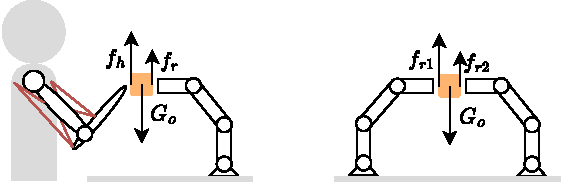
\includegraphics[width=0.8\linewidth]{Papers/images/carrying_schema.pdf}
    \caption{Illustrative example of collaborative object carrying in two different collaborative scenarios, human-robot collaboration on the left and dual robot arm collaboration on the right.}
    \label{fig:carrying_schema}
\end{figure}

One traditional example of a collaborative task requiring physical interaction between multiple actors (humans and robots) is collaborative object carrying~\cite{Arai2000carrying,Kosuge1997carrying,Tsumugiwa2002carrying}. In this task $N$ actors collaborate physically by applying forces $\bm{f}_{a_i}$ on the object with mass $m$, in order to compensate for its gravity $G$
\begin{equation}
    G=m\bm{g}=\bm{f}_{a_1} + ~\cdots ~+\bm{f}_{a_N}
\end{equation}
An illustration of the human-robot and dual robot arm collaborative carrying is given on \Cref{fig:carrying_schema}. As discussed in \Cref{ch:collab_metrics}, in this particular collaboration scenario, each of the actors' capacity to generate forces $\bm{f}_{a_i}$ can be expressed in the polytope form
\begin{equation}
    \bm{f}_{a_i} \in \mathcal{P}_{f,a_i}
\end{equation}
while their joint capacity of generating the forces on the object can be found as the Minkowski sum of their polytopes
\begin{equation}
    \mathcal{P}_f = \mathcal{P}_{f,a_1} \oplus~\cdots~\oplus \mathcal{P}_{f,a_N}
\end{equation}
Therefore if gravity induced force acting the object $G$ is within the polytope $\mathcal{P}_f$ the collaborative system is able to compensate for the objects weight
\begin{equation}
    G \in \mathcal{P}_f
\end{equation}
As both human's and robot's force capacity is state dependant\footnote{The human's and the robot's state force capacity is dependant on their respective states. The exact relationships are described in \Cref{ch:poly_force} for robots and in \Cref{ch:force_poly_human} for humans.} and changes during the execution of the task, the role of the robot control strategies is to find the suitable forces $\bm{f}_{a_i}$ that respect their individual capacities $\mathcal{P}_{f,a_i}$ and accomplish the task by compensating for the object's weight $G$. 

The following two sections present two different robot control strategies for two different collaborative object carrying scenarios. \Cref{ch:robot_robot_carrying} brings a physical collaboration scenario based on two robotic arms carrying an object with a mass of 12kg. Their physical abilities are calculated in real-time in the polytope form and integrated in the real-time robot control in order to exploit their full force capacity. \Cref{ch:human_robot_carrying}, on the other hand, proposes the human-robot physical collaboration scenario for carrying of an object with the mass of 7kg. In this scenario, both of their physical abilities are evaluated online and used to create a human-centred robot control strategy, able to exploit their changing physical abilities while ensuring their safety. 


\section{Dual robotic arm collaborative object carrying}
\label{ch:robot_robot_carrying}

\begin{figure}[!h]
    \centering
    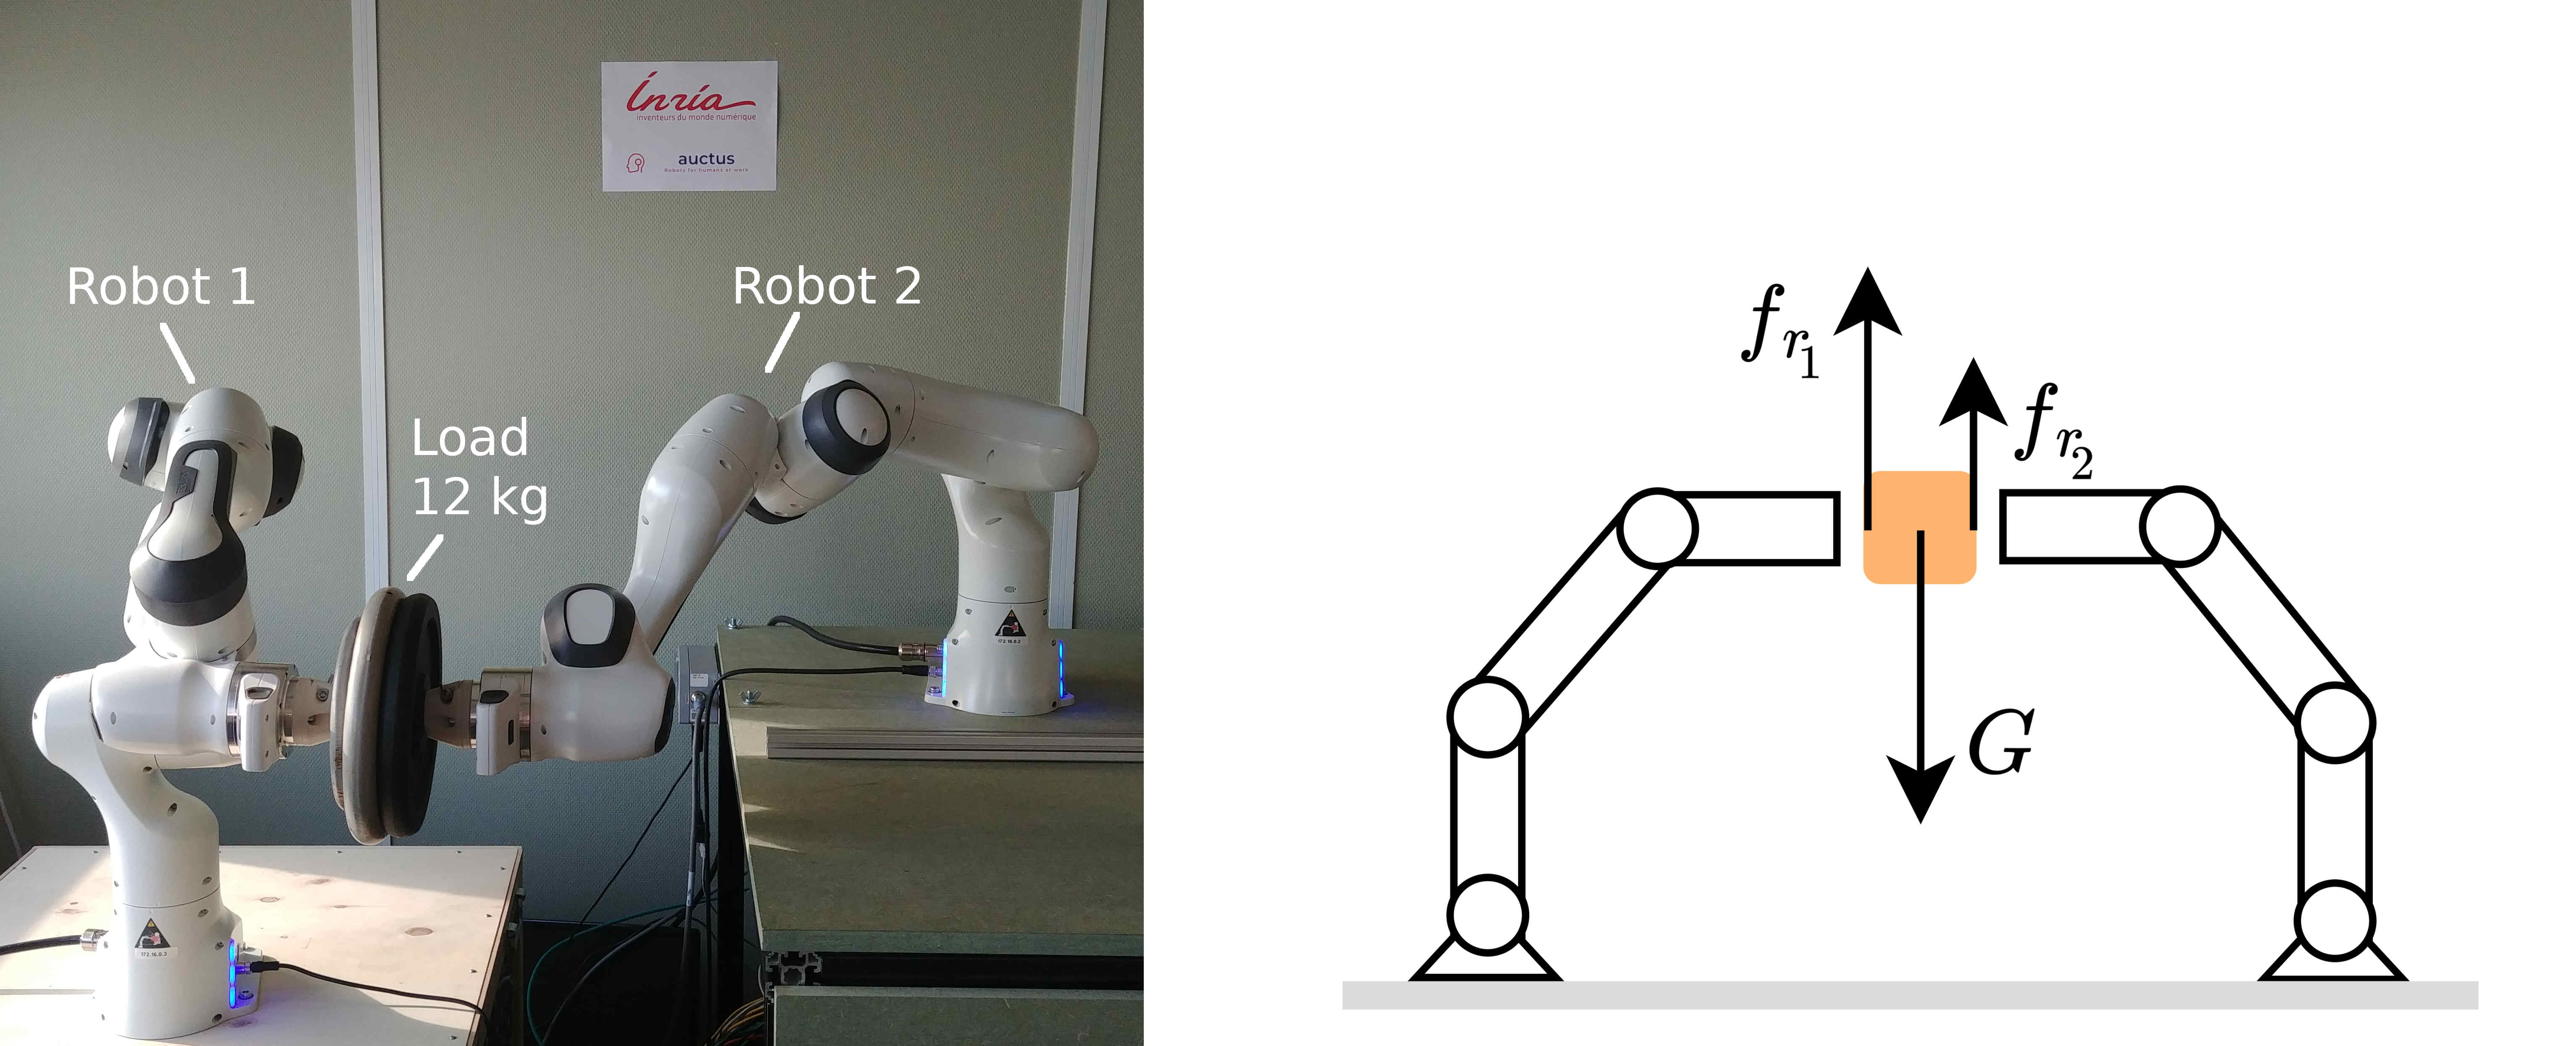
\includegraphics[width=0.9\linewidth]{Papers/images/real_robots_schema_exp1.jpg}
    \caption{Figure showing the experimental setup for dual robot arm collaborative carrying. Two Franka Emika Panda robots jointly carry the object with a mass of $m=12$kg, where each object compensates for a part of the total weight $\bm{f}_{r_1} + \bm{f}_{r_2} = m\bm{g}$. The object is rigidly fixed in the end-effectors of both robots.}
    \label{fig:exp1_real_schema}
\end{figure}


This sections presents a physical collaboration scenario using two {Franka Emika Panda} robots involved in the collaborative carrying on an object of mass $m$. Each robot is contributing to the compensation of the object's gravity $G=m\bm{g}$ by producing forces $\bm{f}_{r_1}$ and $\bm{f}_{r_2}$, such that
\begin{equation}
    \bm{f}_{r_1} + \bm{f}_{r_2} = G
\end{equation}

Panda robots are rated to a maximal carrying capacity of 3kg, which corresponds to the absolute minimal carrying capacity of the robot, evaluated in one of its near-singular configurations. It is, by definition, an underestimation of the real robot's task space force capacity and relying on it, as it is commonly done, limits the scope of the possible tasks and applications.

The goal of this experiment is to demonstrate the fact that by taking into account the true force capacity of each robot, it is possible to go considerably beyond the robot's conservative rated capacity without comprising safety nor exceeding any of the actuation limits\footnote{It it worth noting that the mechanics of the robot's joints might not be designed to withstand the efforts above its rated payload in the long-run. However, this experiment aims to illustrate an optimised use of the robot's abilities, assuming perfectly rigid joints in the directions producing no motion.}. The weight of the object chosen for the experiments is $m=12kg$, voluntarily far above the recommended joint carrying capacity $ m\le 6kg$. 

The following \Cref{sec:robot_carrying_capacity} proposes an efficient approach for calculating the carrying capacity of both robots, leveraging the efficiency of the VEPOLI$^2$ algorithm (described in \Cref{sec:algorithm_vea}). \Cref{sec:collab_robot_control_double_robot} proposes a robot control strategy exploiting this real-time information in order to fully compensate for the continuous evolution of their capacity over time. Finally, \Cref{sec:experiment_dual_robto_carrying} brings the experimental validation of the approach, as well as the discussion of the results. 

\subsection{Robot carrying capacity calculation}
\label{sec:robot_carrying_capacity}


As the carrying task requires the robots to apply only the forces $f_{r_1}$ and $f_{r_2}$ that are opposite to the force of the object's gravity $G$, their physical ability to carry certain weight can be evaluated as the maximal applicable force in the vertical ($z$-axis) direction. Therefore, the robot's carrying capacity $\mathcal{F}_z$ can be expressed as the the special case of the robot's wrench polytope $\mathcal{P}_{f}$, described in \Cref{ch:poly_force}, where the task space is one dimensional ($m=1$)
\begin{equation}
    \mathcal{F}_z (\bm{q},\dot{\bm{q}}) = \mathcal{P}_{f_z} (\bm{q},\dot{\bm{q}}) = \{ f \in \mathbb{R} ~|~ J_{z}(\bm{q})^Tf=\bm{\tau} - \bm{\tau}_b(\bm{q},\dot{\bm{q}}), \quad \bm{\tau}\in[\bm{\tau}_{min}, ~\bm{\tau}_{max}]\}
\end{equation}
where $\{\bm{q},\dot{\bm{q}}\}$ is the robot's joint state, $f \in\mathbb{R}$ is the applicable scalar force in $z$-axis direction, $\bm{\tau}\in\mathbb{R}^n$ are the applied joint torques limited within the interval $\bm{\tau}\in[\bm{\tau}_{min}, ~\bm{\tau}_{max}]$, $\bm{\tau}_{b}\in\mathbb{R}^n$ are the bias joint torques grouping the effects of gravity and robot's motions, while $J_{z}\in\mathbb{R}^{1\times n}$ is the configuration dependant Jacobian matrix with one line and $n$ columns.

\begin{wrapfigure}[14]{r}{0.35\linewidth}
\vspace{-0.5cm}
    \centering
    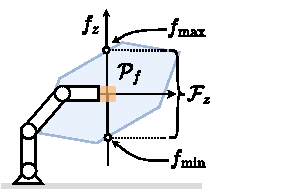
\includegraphics[width=\linewidth]{Papers/images/carrying_capacity_robot.pdf}
    \caption{A geometric view of constructing the carrying capacity $\mathcal{F}_z$ as the intersection of the force polytope $\mathcal{P}_f$ and the $z$-axis. The carrying capacity is expressed at the center of the object.}
    \label{fig:carrying_cap_robot}
\end{wrapfigure}

Geometrically, the $m=1$ dimensional polytope, describing the range of scalar forces $f$ applicable in the vertical direction, can be represented as the intersection of the complete wrench/force ($m=6$/$m=3$) polytope $\mathcal{P}_f$, described in \Cref{ch:poly_force}, with the vertical axis. An illustrative view of this intersection is shown on \Cref{fig:carrying_cap_robot}.

For any given robot state $\{\bm{q},\dot{\bm{q}}\}$ this one dimensional set $\mathcal{F}_z$ can be transformed into the form of a min-max interval
\begin{equation}
    \mathcal{F}_z = \{ f \in \mathbb{R} ~|~ f \in[{f}_{min}, ~{f}_{max}]\}
\end{equation}
Finding the limits $[f_{min},~f_{max}]$ of the applicable scalar force $f$ in the vertical direction can be viewed as finding a $\repr{V}$-representation of the 1D ($m=1$) polytope $\mathcal{F}_z$. Then the vertex search algorithm VEPOLI$^2$, described in \Cref{sec:algorithm_vea}, can be used to efficiently find the limits (vertices) $f_{min}$ and $f_{max}$ of the applicable force in $z$-axis direction.  

Furthermore, this procedure can be done for both robots $r_1$ and $r_2$, by characterising their carrying capacities
 $\mathcal{F}_{z,r_1}$ and $\mathcal{F}_{z,r_2}$ and finding their applicable vertical force ranges 
\begin{equation}
    f_{r_1} \in [f_{r_1,min}, ~f_{r_1,max} ], \quad f_{r_2}\in [f_{r_2,min}, ~f_{r_2,max}]
    \label{eq:robot_robot_carrying_capacity}
\end{equation}
 
Additionally, their combined carrying capacity $\mathcal{F}_{z,r_1+r_2}$ can be calculated as the Minkowski sum of their polytopes $\mathcal{F}_{z,r_1}$ and $\mathcal{F}_{z,r_2}$ 
$$\mathcal{F}_{z,r_1+r_2} = \mathcal{F}_{z,r_1}\oplus \mathcal{F}_{z,r_2}$$
or in this special case ($m=1$), the sum of their intervals 
$$f_{r_1+r_2} = f_{r_1}+f_{r_2} \in  [f_{r_1,min} + f_{r_2,min}, ~f_{r_1,max} + f_{r_2,max}].$$

In the context of this experiment, the real-time carrying capacity calculation is implemented using the Python open-source library \codet{pycapacity}, developed in the context of this thesis and described in \Cref{ch:software}.

\subsection{Collaborative robot control strategy}
\label{sec:collab_robot_control_double_robot}
The collaborative carrying task requires the robot's to apply forces that compensate for the object's weight $G$, which can be expressed in a form
\begin{equation}
    f_{r_1} + f_{r_2} - G = 0
    \label{eq:robot_robot_weight_compensation}
\end{equation}

In the general case, there exists an infinity of ways the weight can be distributed between the two robots, satisfying equation (\ref{eq:robot_robot_weight_compensation}) and, at the same time, respecting their carrying capacities $\mathcal{F}_{z,r_1}$ and $\mathcal{F}_{z,r_2}$.

In this work, a simple weight distribution strategy is proposed, where the relative load of each of the robots, with respect to their carrying capacity is evenly distributed. 
\begin{equation}
\frac{f_{r_1}}{f_{r_1,max}} = \frac{f_{r_2}}{f_{r_2,max}}
\label{eq:ratio_robot_constant}
\end{equation}
In other words, the weight the robot carries is proportional to its carrying capacity. Combining equations (\ref{eq:robot_robot_weight_compensation}) and (\ref{eq:ratio_robot_constant}), the weight carried by each one of the robots can be expressed as
\begin{equation}
f_{r_1} = \underbrace{\frac{f_{r_1,max}}{f_{r_1,max} + f_{r_2,max}}}_{\lambda_1} G, \qquad f_{r_2} = \underbrace{\frac{f_{r_2,max}}{f_{r_1,max} + f_{r_2,max}}}_{\lambda_2}G 
\label{eq:robot_robot_weight_distribution}
\end{equation}
where $\lambda_1$ and $\lambda_2$ represent the ratios of both robot's contribution to the overall carrying capacity, and their relationship can be expressed as $\lambda_1 + \lambda_2 = 1$.

In order to find the optimal forces $f_{r_1}$ and $f_{r_2}$ that, at the same time, compensate for the weight of the object (\ref{eq:robot_robot_weight_compensation}), comply with the proposed weight distribution strategy (\ref{eq:robot_robot_weight_distribution}) and respect their carrying capacities (\ref{eq:robot_robot_carrying_capacity}), a \gls{qp} based robot control strategy is proposed
\begin{equation}
\begin{split}
    f_{r_1}, f_{r_2} = \underset{f_{r_1},f_{r_2}}{\arg\min} &~\overbrace{||G - f_{r_1} -f_{r_2}||^2}^{\text{weight compensation}} ~~+ \overbrace{ \omega\lambda_2||f_{r_1}||^2 + \omega\lambda_1||f_{r_2}||^2}^{\text{weight distribution}}\\
    s.t.& \quad f_{r_1} \in[f_{r_1,min}, f_{r_1,max}]\\
    & \quad f_{r_2} \in[f_{r_1,min}, f_{r_2,max}]\\
\end{split}
\label{eq:qp_robot_robot}
\end{equation}

The proposed optimisation problem consists in two tasks. The first task is the weight compensation task, corresponding to equation (\ref{eq:robot_robot_weight_compensation}), which is ensured by minimising the error $||G - f_{r_1} -f_{r_2}||^2$. Expressing equation (\ref{eq:robot_robot_weight_compensation}) in this form, allows for the cases when the robot's carrying capacities are not sufficient for carrying the object $f_{r_1,max} + f_{r_2,max}<G$. Preventing such situations and ensuring the feasibility of the robots' tasks presents a substantial research challenge in the realm of robot task design. 

In the context of collaborative carrying task, a potential avenue in addressing this issue comes from wrench feasibility analysis \cite{gouttefarde2006determination,Lau2011}. These tools could enable quantifying the areas of the collaborative workspace, where a certain weight compensation capacity is guaranteed. Then, the collaborative carrying tasks could be designed within these ares in the workspace. It's worth noting that these approaches complement the proposed approach and could be used in tandem to further improve the robustness of the proposed method and bring it a step closer to practical real-world applications.  

\begin{figure}[!b]
    \centering
    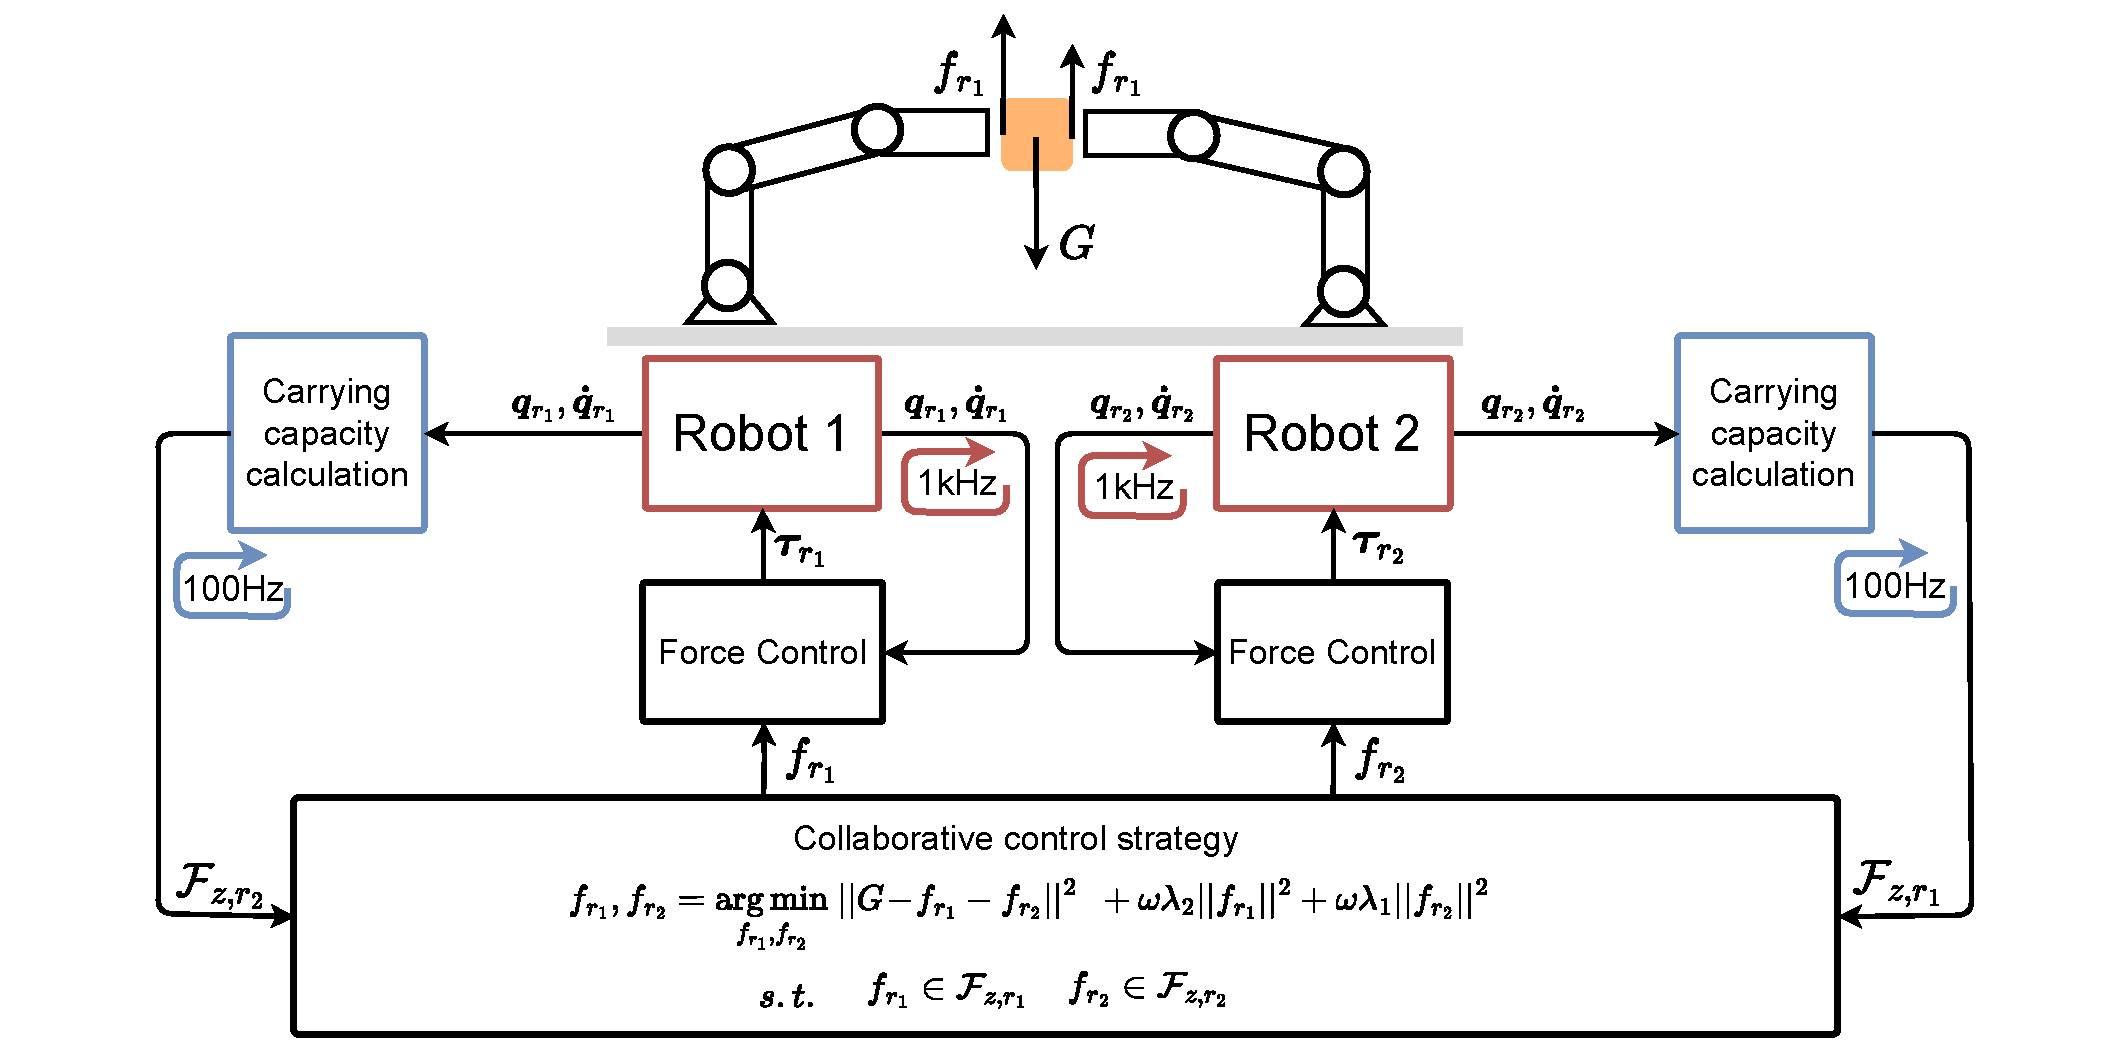
\includegraphics[width=\linewidth]{Papers/images/schema_robot_robot.pdf}
    \caption{The block diagram showing the implemented robot control scheme. Each robot's low-level force control loop runs at 1kHz, while the carrying capacity calculation and the collaborative control strategy are evaluated at the frequency of 100Hz.}
    \label{fig:schema_robot_robot_control}
\end{figure}


The second task ensures the even relative load distribution between the robots, as proposed by the weight distribution strategy given in equation (\ref{eq:robot_robot_weight_distribution}). To achieve this behaviour, the norm of the first robot's force $f_{r_1}$ is weighted by the second robot's contribution ratio $\lambda_2$, while the second robot's force $f_{r_2}$ is weighted by the first robot's contribution ratio $\lambda_1$. This way, if the robot $r_1$ has higher carrying capacity $f_{r_1,max}>f_{r_2,max}$, the force $f_{r_1}$ is weighted (penalised) less in the cost function $\lambda_1>\lambda_2$, ultimately resulting in higher values found by the optimisation problem for robot 1. On the other hand, if the carrying capacities of both robots is equal, then the weighing factors are equal too $\lambda_1=\lambda_2$, resulting in the equal weight distribution. 

The factor $\omega$ is used to set the priority of the weight distribution task much lower than the main task of the weight compensation of the object, in the experiments proposed in this sections the regularisation weight is set to $\omega=1\times 10^{-5}$.

Each robot control cycle starts by calculating the carrying capacities (\ref{eq:robot_robot_carrying_capacity}), followed by the resolution of the optimisation problem (\ref{eq:qp_robot_robot}). Once the optimal vertical forces $f_{r_i}$, are obtained the joint torques $\bm{\tau}_{r_i}$, achieving those forces, are calculated for each of the robots and sent to their low-level joint controllers 
\begin{equation}
    \bm{\tau}_{r_i} = J_{z,r_i}^T(\bm{q}_{r_i}){f}_{r_i} + \bm{\tau}_{b,r_i}(\bm{q}_{r_i},\dot{\bm{q}}_{r_i}), \qquad \forall i \in \{1,2\}
\end{equation}

The calculation of the carrying capacity of both robots and the proposed collaborative control strategy are implemented in programming language Python and performed at the frequency of 100Hz.  The robot's open-loop force control is implemented in programming language C++, using the library \codet{pinocchio}~\cite{pinocchio2021}, and run at the frequency of 1kHz. The complete software stack has been integrated using the \gls{ros}~\cite{ros} programming environment and run from one computer equipped with a 1.90GHz Intel i7-8650U processor. 
\Cref{fig:schema_robot_robot_control} shows the schematic block diagram of the implemented collaborative robot control strategy. 

\subsection{Experimental validation}
\label{sec:experiment_dual_robto_carrying}
\begin{figure}[!h]
    \centering
    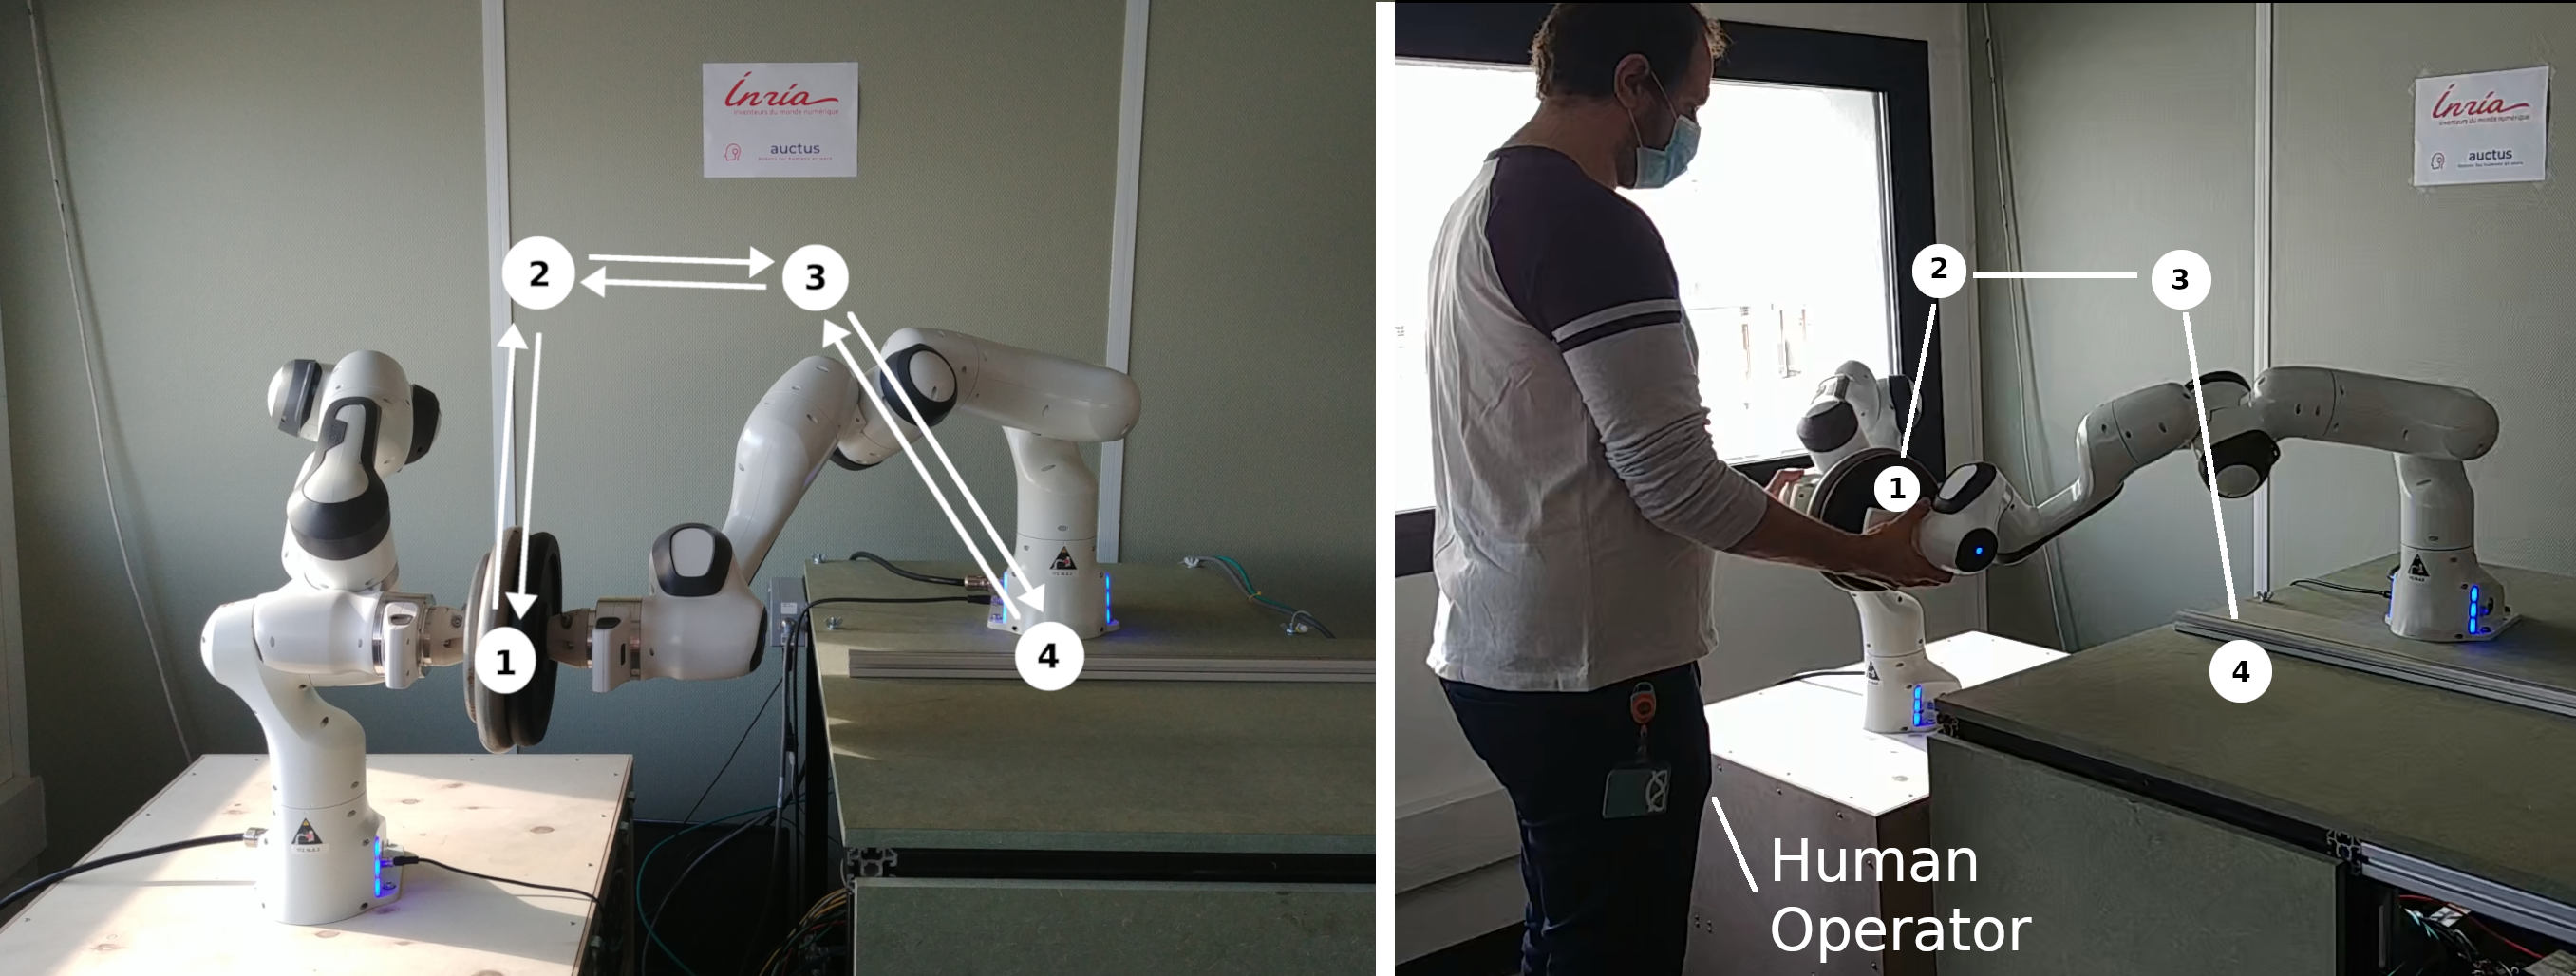
\includegraphics[width=\linewidth]{Papers/images/exp1_explication.jpg}
    \caption{This figure shows the experimental setup and visualises the trajectory taken by the human operator. The robots compensate for the full object's weight while the operator moves the object through the workspace, doing a forward and backward pass through the 4 via-points.}
    \label{fig:experiment1}
\end{figure}

\qrimg{qrcodes/icra2021.png}{https://youtu.be/hApIv1oFuhk}{Video}
In this experiment the two Panda robots jointly compensate for the weight of the object (12 kg), using the proposed collaborative control strategy. A human operator freely moves the object through the common work-space, implicitly changing both robots' configurations in real-time. As a consequence, the task space trajectory and the evolution of the robot configurations are not known in advance. 

The particular trajectory taken by the human operator in this experiment is indicated on \Cref{fig:experiment1}. It consists in taking the object through the set of four via-points, making a forward and backward pass. The proposed control strategy then leverages the real-time calculation of their carrying capacity and adapts the weight distribution to ensure the compensation of the full object's weight during the whole experiment. 

\afterpage{
\begin{landscape}
\begin{figure}
    \centering
    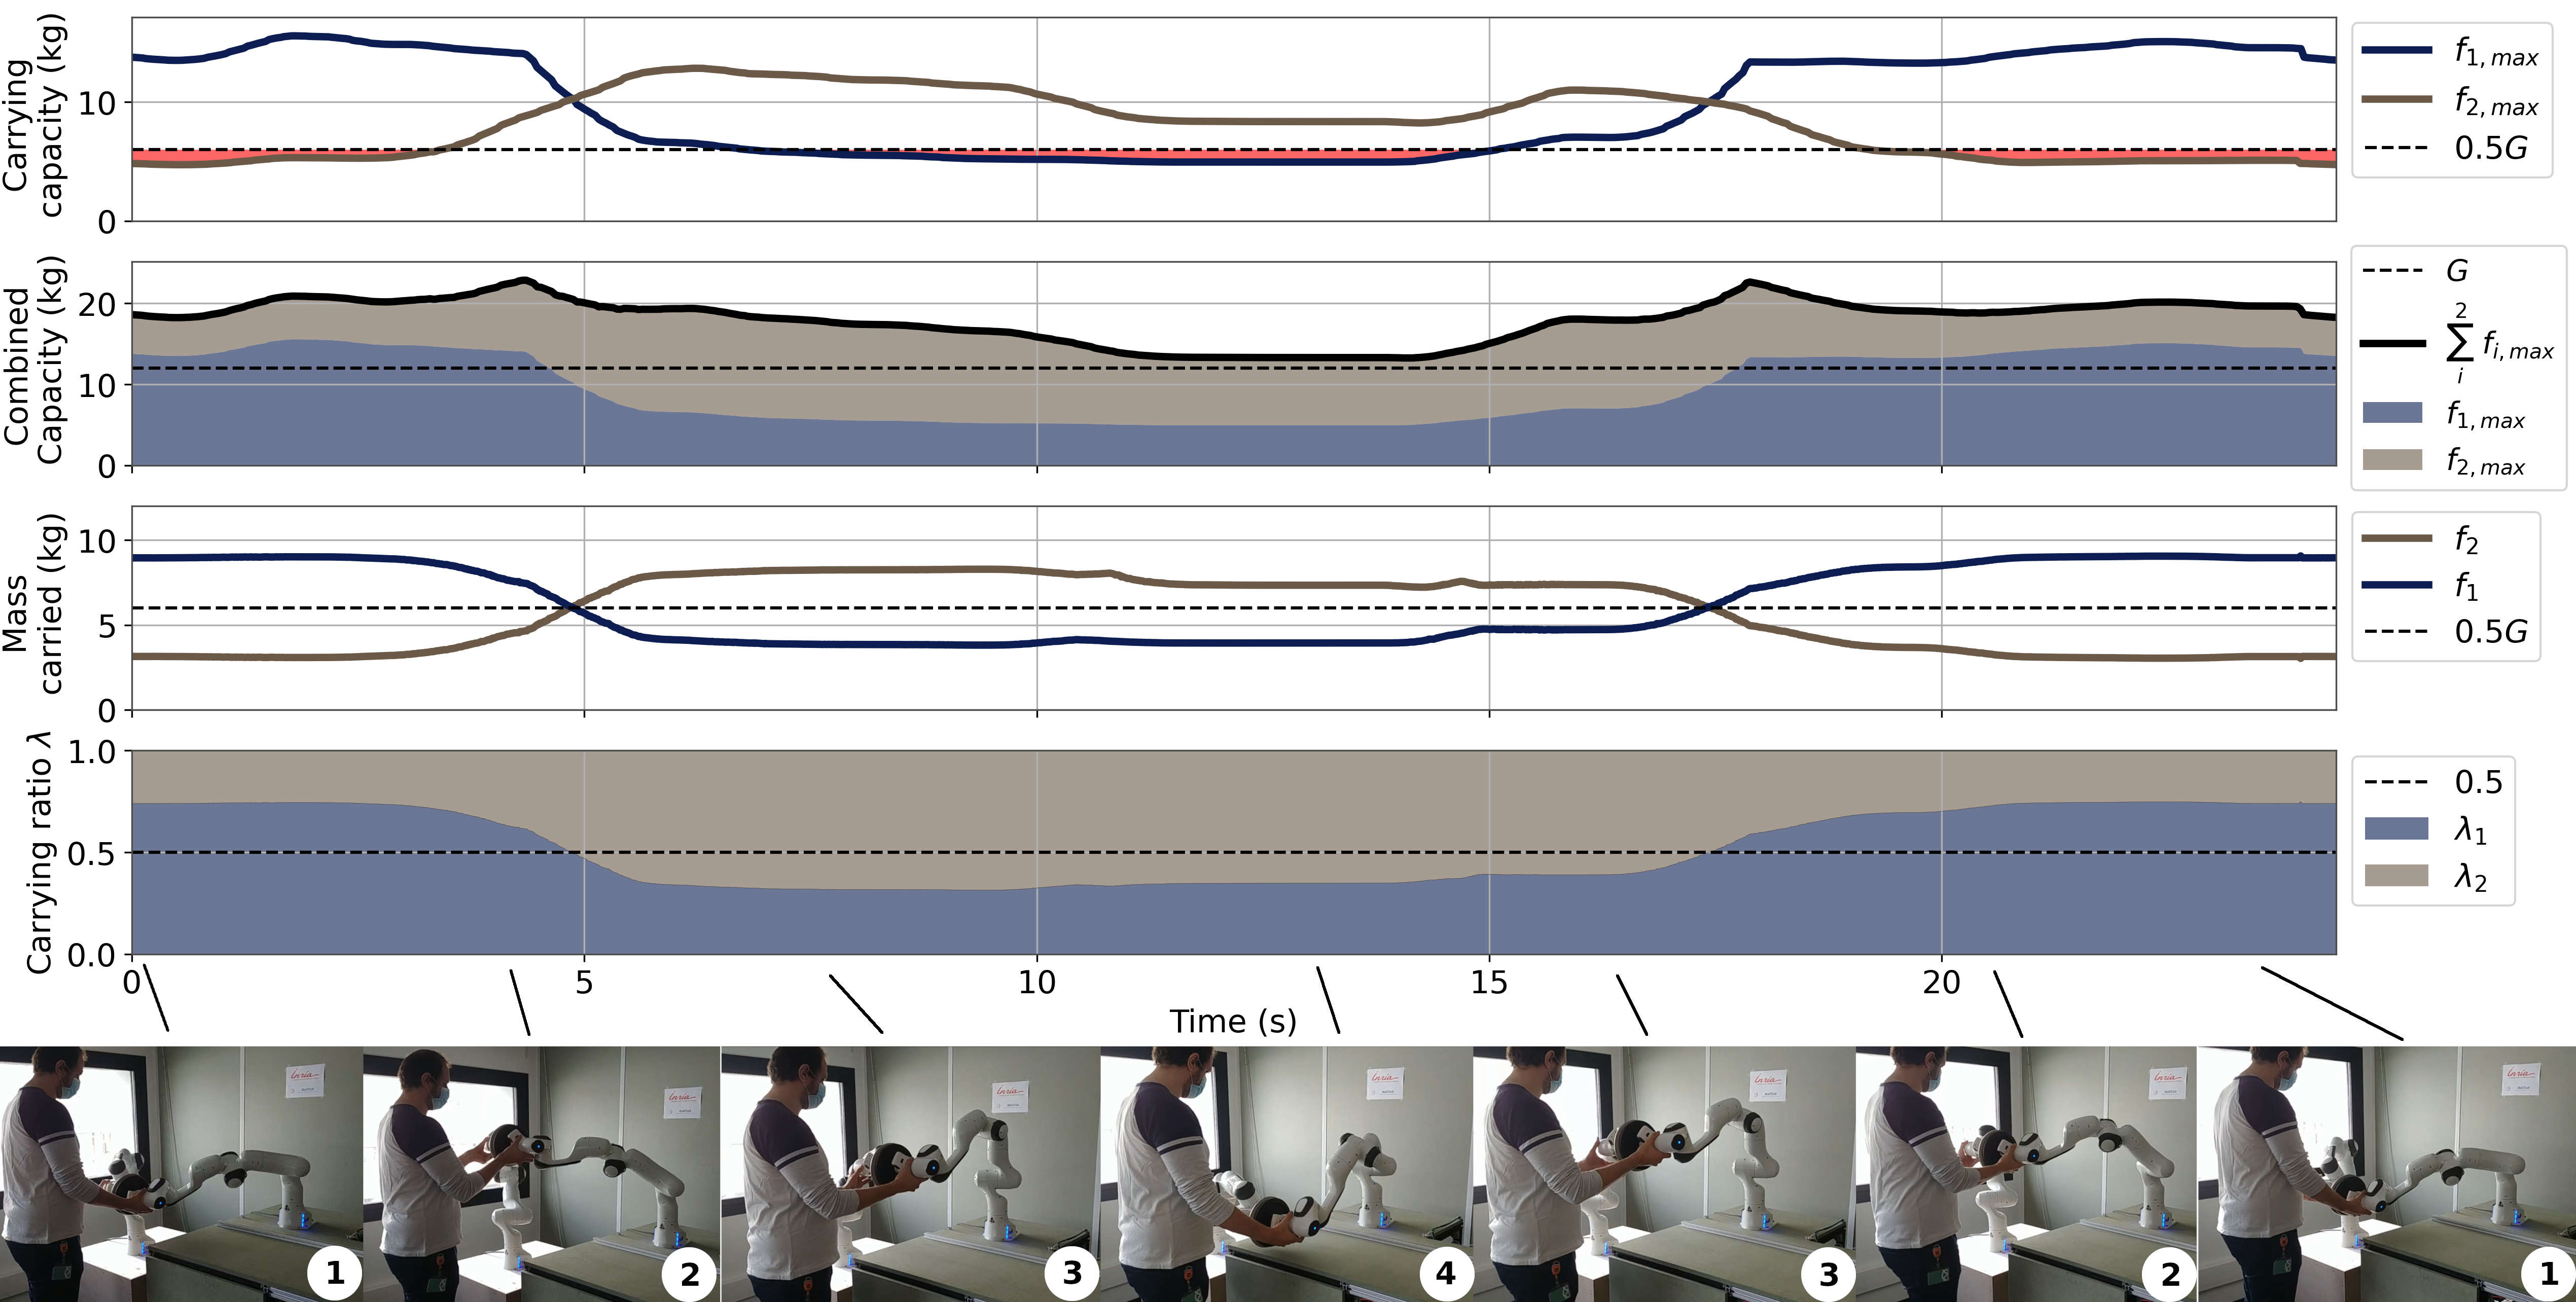
\includegraphics[width=\linewidth]{Papers/images/exp_no_anim.jpg}
    \caption{This figure shows the time evolution of different control and physical ability variables in the top graphs, as well as several images of the experiment taken when the operator attained different via-points with the object. 
   The top graph shows the time evolution of the carrying capacity of the manipulators $f_{r_1,max},f_{r_2,max}$, indicating, with red background, the time periods when the naive strategy $f_{r_1}=f_{r_2}=0.5G$ (dashed line on all graphs) would not be feasible for at least one of the two robot. 
   The second  graph provides the evolution of their joint capacity $f_{max}=f_{r_1,max}+f_{r_2,max}$, indicating their individual contributions to the common capacity. The third graph indicates the time evolution of applied manipulator forces $f_{r_1}, f_{r_2}$, calculated using the proposed control strategy. Finally, the bottom graph shows the time evolution the weights $\lambda_1,\lambda_2$ used with the robot control. All the force values are expressed in kilograms for easier readability.     
    }
    \label{fig:dual_manip}
\end{figure}
\end{landscape}
}

A straightforward control strategy, requiring each robot to compensate for half of object mass $f_{r_1}=f_{r_1}=0.5G$ is taken as baseline to evaluate the performance of the new method. This experiment is illustrated in the accompanying video\footnote{Video: \url{https://youtu.be/hApIv1oFuhk}}.

\Cref{fig:dual_manip} (bottom) shows several images taken during the experiment execution, in the moments when the operator reached different via-points. The graphs on the top show the time evolution of the evaluated maximal forces and force applied by each robot during the experiment. The naive strategy $f_{r_1}=f_{r_1}=0.5G$ is shown in dashed lines for comparison. 


The results show that the proposed control strategy is successful in ensuring compensation of the object weight during the full length of the experiment. In the starting via-point $t=0$s and $t\geq21$s, robot $r_2$ (robot on the right) is close to it's singular configuration and its load carrying capacity is close to $5$kg. Controlling it to compensate for half of the weight of the object would result in a saturation of the actuators and potential damage to the hardware. The same is true for via-point 4 at $t=12$s. In this via-point the robot $r_1$ (robot on the left) is not be able to compensate for half of the object weight, but thanks to the proposed adaptive control law, the task can successfully be achieved, supporting \Myref{hyp:individual_capacity}. 
Furthermore, any naive fixed strategy, assigning certain fixed ratio of the object's weight to the robots, would result in surpassing the robots' limits which in turn would fail to accomplishing the task. 
By exploiting the online calculation of the robots' physical abilities, the proposed strategy enables exploiting their changing abilities and accomplishing this task while at the same time guaranteeing that their capacities are not exceeded. 

The results further show that even though in the large portion of the experiment one of the robots was not able to carry half of the object's weight, their joint carrying capacity exceeded the objects weight $f_{r_1,max}+f_{r_2,max} >G$ during the whole length of the experiment, conforming with \Myref{hyp:common_capacity}.

However, this may not be the case over the entire common workspace of the two robots, but this example is a good illustration of the interest of accounting for the true capabilities of the system at the control level.  In certain configurations the common carrying capacity of the robots might be lower than the objects weight $f_{r_1,max}+f_{r_2,max} <G$. The proposed control approach, in those cases would ensure that the robots' physical abilities are not exceeded, however it would not be able to guarantee the weight compensation of the object. 

In summary, the experimental validation demonstrates the effectiveness of the proposed control strategy in real-time adaptation of weight distribution between multiple robots based on their varying physical abilities. The strategy ensures safe and efficient collaboration between robots, allowing them to collectively perform tasks that would be challenging or impossible for each robot to accomplish individually. Leveraging real-time information about their physical abilities, the proposed strategy offers a flexible solution for collaborative applications, eliminating the need for pre-calibration or in advance task-specific information.

\section{Human-robot collaborative object carrying}
\label{ch:human_robot_carrying}

\begin{figure}[!h]
    \centering
    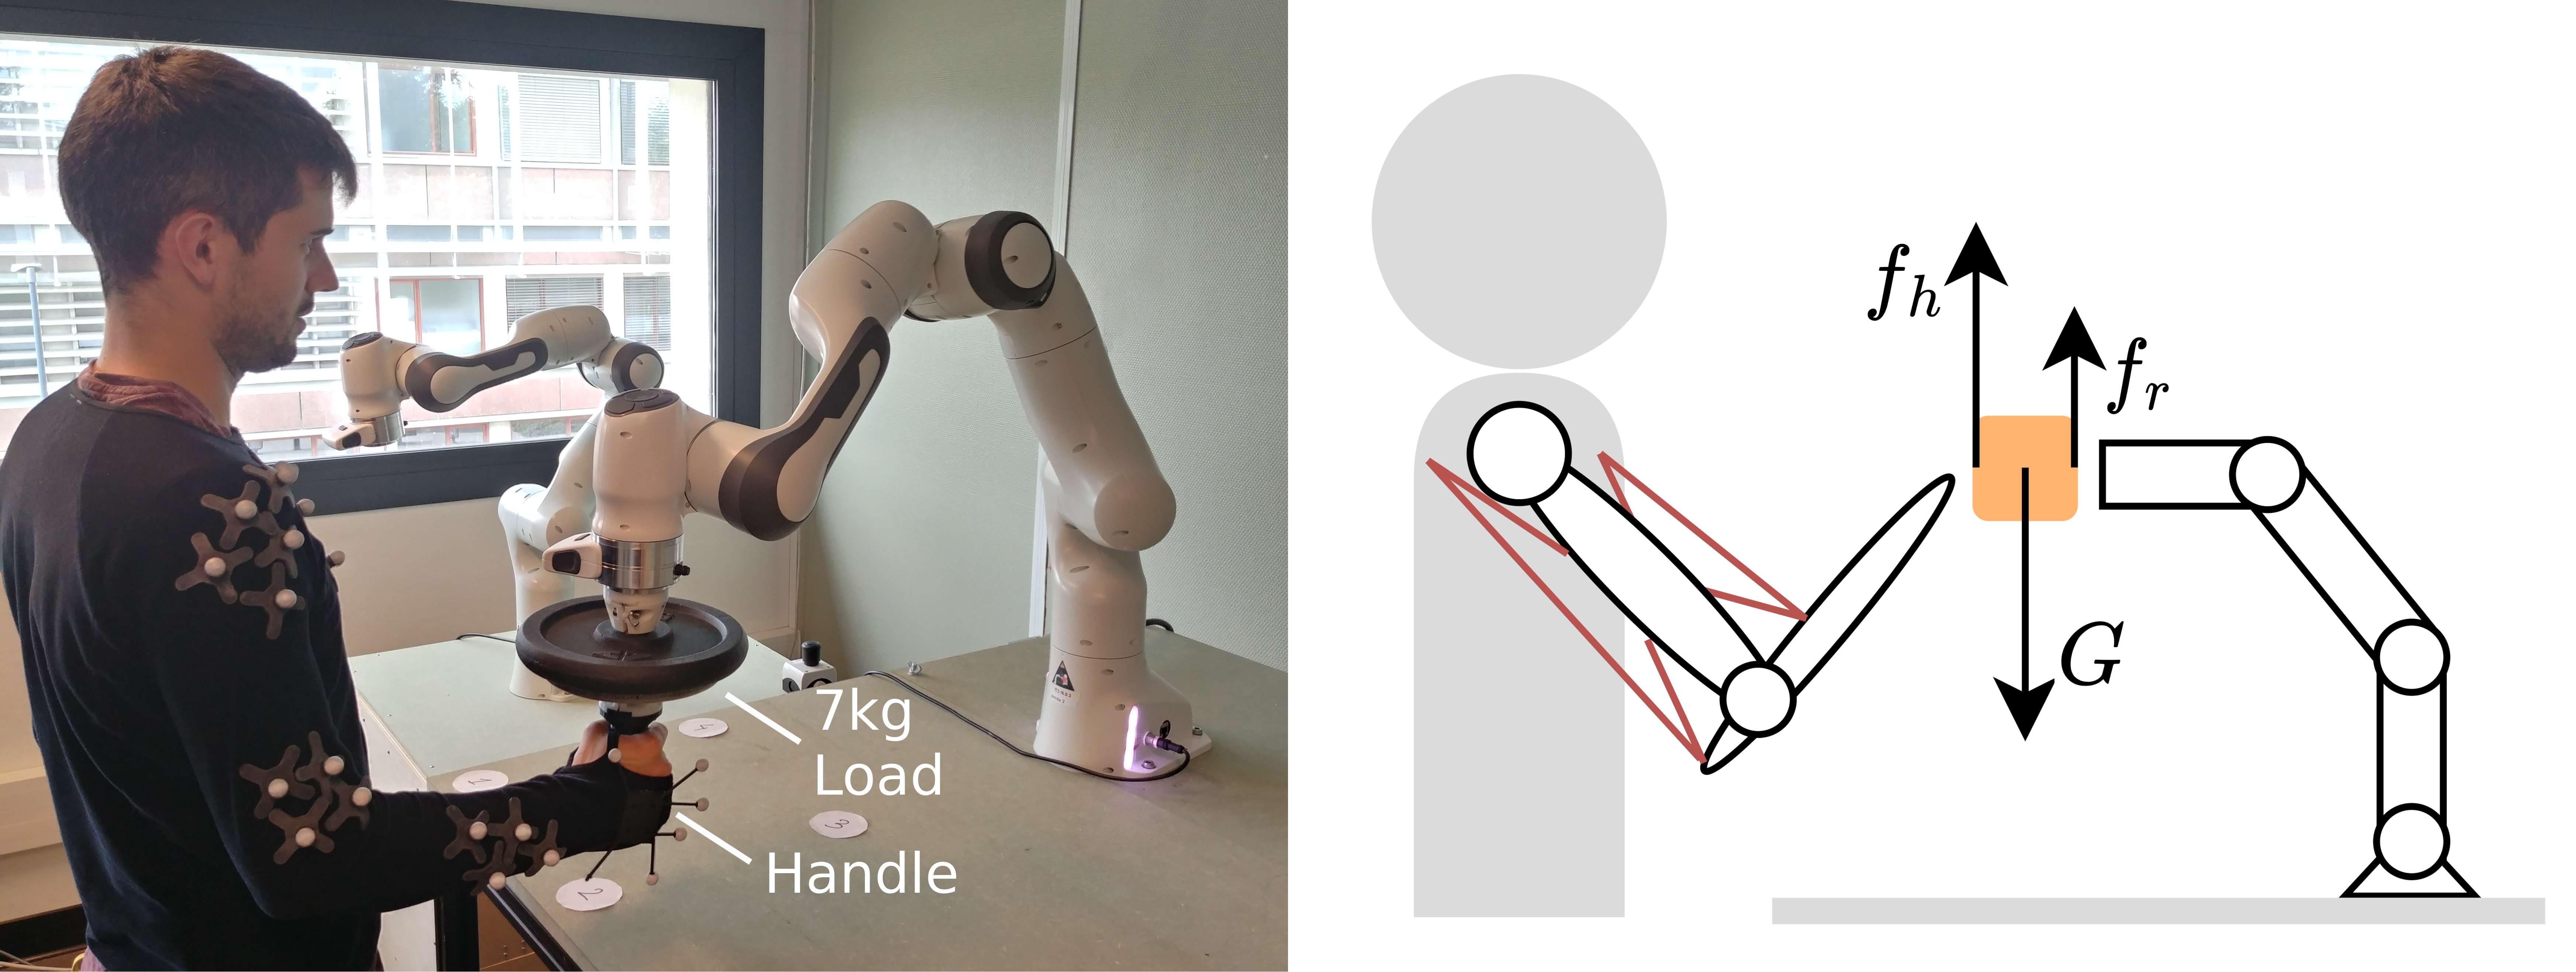
\includegraphics[width=0.9\linewidth]{Papers/images/exp2_real_schema.jpg}
    \caption{This figure show the experimental setup. The robot end-effector is fixed to the carried object and the human operator is holding the object by the handle. The object's mass is $m=7$kg, while the operator and the robot collaborate to compensate the full weight of the object.}
    \label{fig:exp2_real_schema}
\end{figure}

In many industrial contexts, including the LiChiE project's mini-satellite fabrication process, tasks involving the manipulation of heavy objects are a frequent occurrence. 
Taking inspiration from these tasks, this section presents an illustrative scenario where a human and a robot collaborate physically to carry a heavy object. In this scenario, shown on \Cref{fig:exp2_real_schema}, a human operator and a {Franka Emika Panda} robot jointly carry an object mass of $m\!=\!7$ kg, each one compensating for a part of the total weight 
\begin{equation}
    \bm{f}_h  + \bm{f}_r = m\bm{g} = G
\end{equation}

In this experiment, the operator has the expert knowledge about the task and moves the object through the workspace to perform the task efficiently. The robot's role, in this case, is to assist the operator with the carrying of the heavy object and improve their safety and their overall well-being.

The usual choice for these scenarios is a simple gravity compensation strategy, making the robot carry the full weight of the object $\bm{f}_r = G$ and provide the operator with full movement transparency. Several such human-centred robot control strategies have recently been proposed in the literature, where the robot in addition to the full weight compensation improves different aspects of the human safety and ergonomics. One example of such approach is proposed by \citet{ferraguti2020unified}, which REBA \cite{reba} ergonomic indicators to improve human posture while carrying an object. 

However, as discussed in \Cref{ch:robot_robot_carrying}, assigning any fixed weight to the robotic manipulator requires \textit{a priori} analysis of its changing capacity and determination of the \textit{worst-case} weight limits, which in the case of the Franka Emika Panda robot is $m\leq3$kg\footnote{Given by the manufacturer in the form of the robot's rated payload.}. Therefore, carrying the 7kg load requires using a more capable robot which, in many cases, significantly increase the cost of such system and potentially reduces operator's safety. As more capable robots are usually bigger and heavier, they result in much higher exchanged forces in case of impact with the operator, raising many safety concerns~\cite{smu}.
Therefore, delegating the entire weight compensation to the robot is not always the most efficient or the safest solution for the operator. 

On the other hand, several studies have shown that the human's physical feedback during task execution improves significantly their engagement in the task \cite{rani2007operator}, improves the task execution efficiency and reduces the risk of error \cite{BYRNE1996249}. However, since the human's carrying capacity varies significantly throughout the workspace as well, before allocating any weight to the operator, their safety has to be ensured. As in the case of robots, the traditional approach consists in analysing the task in advance and determining, often in a very conservative manner, the set of \textit{worst-case} limits \cite{shoaf1997comprehensive}, often given in a form of different standards \cite{nasa} and manuals \cite{health1992manual}. 

In order to avoid making such coarse assumptions, several approaches have been proposed in the literature, able to quantify different measures of human physical abilities and adapt the human load to their changes online. \citet{Kim2018} have proposed an approach estimating the joint torques in the operator's body produced by carrying the load of the object, where the robot's role is to adapt the operator's posture to minimise the magnitude of human's joint torques. The human body is approximated using a planar model actuated at the joint level. Furthremore, in their work, the human is the one carrying the full mass of the object, while the robot's only role of is to modify the operator's posture in order to improve his ergonomics. 

A different approach is proposed by \citet{carmichael2013admittance}, where the human and the robot collaborate physically to execute the carrying task. Their approach is employs on a more accurate human model, based on human musculoskeletal models, which is used to efficiently approximate the human's force capacity. The robot control strategy modulates the weight carried by the human with respect to the approximation calculated in real-time. The approach is developed in the context of human rehabilitation and used for the real-time control of assistive exoskeletons. The authors show that such approach is capable of adapting to the operator's pathology and reduce the rehabilitation time~\cite{Carmichael2013Experimental}. 
This approach demonstrates the potential of using human-centred robot control strategies which are able to adapt the load carried by the human precisely to his varying physical abilities. However due to the intractable computational complexity of the human force capacity calculation proposed by the authors, the scope of their work is limited to relatively simple planar musculoskeletal models. Furthermore, the robot control strategy proposed in their work is aimed to the rehabilitation and the use of assistive exoskeletons, which does not transpose well to more unstructured industrial scenarios.

Inspired by their work, this section aims to further demonstrate the potential of using the real-time knowledge about both robot's and human's physical abilities in the context of collaborative robot control in industrial scenarios. The proposed collaborative robot control strategy leverages the two new algorithms developed in the context of this work, capable of efficiently calculating the force capacity of robots (VEPOLI$^2$ described in \Cref{sec:algorithm_vea}) and humans, based on their musculoskeletal models (ICHM described in \Cref{ch:algorihtm_ichm}). 
Their changing capacities are calculated online and used to create collaborative robot control strategy, capable of both exploiting their full potential and, at the same time, ensure the safety of the operator. 

\Cref{sec:human_carrying_capacity} introduces an efficient strategy for calculating the operator's carrying capacity in real-time. \Cref{sec:collab_robot_control_human_robot} introduces the collaborative robot control strategy using the online information about the operator's carrying capacity, as well as the robot's capacity, described in  \Cref{sec:robot_carrying_capacity}. The experimental validation of this approach is described in  \Cref{sec:human_robot_experiment} as well as the discussion on results.

\subsection{Human carrying capacity calculation}
\label{sec:human_carrying_capacity}

As described in \Cref{ch:human_metrics}, the analysis of human's physical abilities in this work is based on their musculoskeleral models, as the most accurate models of human bodies currently available.
More specifically, as shown on \Cref{fig:exp2_real_schema}, this experiment requires evaluating the operator's ability to carry the object in his right arm. 
Many different human arm musculoskeletal models are proposed and validated in the biomechanics literature \cite{holzbaur2005model,saul2015benchmarking}, as well as different software tools for their analysis \cite{opensim,Bouchard2009}. 
However, choosing an appropriate musculoskeletal, and adapting it to individual characteristics of the operator, is a challenging scientific problem. 

In broad terms, using more detailed musculoskeletal models often leads to more accurate representation of human subjects \cite{sohn2019effects}, but comes with an increase in the computational complexity. 
The computational efficiency of the proposed ICHM algorithm, described in \Cref{ch:algorihtm_ichm}, allows for considering relatively detailed models (even up to 50 muscles) while maintaining interactive execution times. 
Therefore, the analysis in this section assumes having an appropriate and detailed musculoskeletal model of the operator's arm. 

When it comes to the collaborative carrying experiment, the operator is required to apply only the force $f_{h}$ that contributes to compensating the object's gravity $G$. Therefore, the task is effectively one dimensional $m=1$ and his physical ability to carry certain weight can be evaluated as the maximal applicable force in the vertical ($z$-axis) direction. Hence, the human's carrying capacity $\mathcal{F}_z$ can be expressed as the the special case of the human's wrench polytope $\mathcal{P}_{f}$, described in  \Cref{ch:force_poly_human}, where the task space is one dimensional ($m=1$)
\begin{equation}
     \mathcal{F}_z(\bm{q},\dot{\bm{q}}) = \mathcal{P}_{f_z} (\bm{q},\dot{\bm{q}}) = \{ f \in \mathbb{R} ~|~ J_{z}(\bm{q})^Tf=N(\bm{q})\bm{F} - \bm{\tau}_b(\bm{q},\dot{\bm{q}}), \quad \bm{F}\in[\bm{F}_{min}, ~\bm{F}_{max}]\}
\end{equation}
where $\{\bm{q},\dot{\bm{q}}\}$ represent the human's joint state, $f \in\mathbb{R}$ is the applicable scalar force in $z$-axis direction, $\bm{F}\in\mathbb{R}^n$ are the applied muscular forces limited within the interval $\bm{F}\in[\bm{F}_{min}, ~\bm{F}_{max}]$, $\bm{\tau}_{b}\in\mathbb{R}^n$ represents the bias joint torques grouping the effects of the gravity and human's motions, while $J_{z}\in\mathbb{R}^{1\times n}$ is the configuration dependant Jacobian matrix with one line and $n$ columns and $N\in\mathbb{R}^{n\times d}$ is the state dependant moment arm matrix. Values $n$ and $d$ correspond to the number of joints and muscles considered in the musculoskeleral model.

Analogously to the robot's case, human's carrying capacity $\mathcal{F}_z$ is a $m=1$ dimensional polytope, describing the range of scalar forces $f$ applicable in the vertical direction. Geometrically, this polytope corresponds to the intersection of the complete wrench/force ($m=6$/$m=3$) polytope $\mathcal{P}_f$, described in \Cref{ch:force_poly_human}, with the vertical axis. An illustrative view of this intersection is shown on \Cref{fig:carrying_cap_human}.

Furthermore, for any given human's state $\{\bm{q},\dot{\bm{q}}\}$ this one dimensional set $\mathcal{F}_z$ can be transformed into the form of a min-max interval
\begin{equation}
    \mathcal{F}_z = \{ f \in \mathbb{R} ~|~ f \in[{f}_{min}, ~{f}_{max}]\}
\end{equation}
In order to find the limits $[f_{min},~f_{max}]$ of the applicable scalar force $f$ in the vertical direction, this problem can be formulated as finding the $\repr{V}$-representation of the 1D ($m=1$) polytope $\mathcal{F}_z$. Then the real-time capable algorithm ICHM, proposed in \Cref{ch:algorihtm_ichm}, can then be used to find the limits (vertices) $f_{min}$ and $f_{max}$ of the applicable force in $z$-axis direction.  


\begin{wrapfigure}{r}{0.4\linewidth}
    \centering
    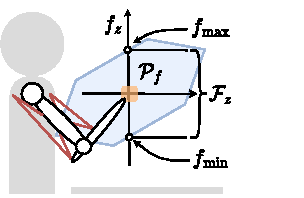
\includegraphics[width=\linewidth]{Papers/images/carrying_capacity_human.pdf}
    \caption{A geometric view of constructing the carrying capacity $\mathcal{F}_z$ as the intersection of the force polytope $\mathcal{P}_f$ and the $z$-axis. The carrying capacity is expressed at the center of the object.}
    \label{fig:carrying_cap_human}
\end{wrapfigure}
Following the similar procedure as for humans, the robot's carrying capacity can be determined in real-time as well, using the VEPOLI$^2$ algorithm, as proposed in \Cref{sec:robot_carrying_capacity}. Then the human's carrying capacity $\mathcal{F}_{z,h}$ and robot's carrying capacity $\mathcal{F}_{z,r}$, characterising their feasible ranges of applicable vertical forces $f_r$ and $f_h$ can be expressed as in the form of ranges
\begin{equation}
    f_{h}\in [f_{h,min}, ~f_{h,max}], \qquad f_{r} \in [f_{r,min}, ~f_{r,max} ]
    \label{eq:human_robot_carrying_capacity}
\end{equation}

Additionally, their combined carrying capacity $\mathcal{F}_{z,h+r}$ can be calculated as the Minkowski sum of their carrying capacities $\mathcal{F}_{z,h}$ and $\mathcal{F}_{z,r}$ 
$$\mathcal{F}_{z,h+r} = \mathcal{F}_{z,h}\oplus \mathcal{F}_{z,r}$$
or in this special ($m=1$), the sum of the intervals 
$$f_{h+r} = f_{h}+f_{r} \in  [f_{h,min} + f_{r,min}, ~f_{h,max} + f_{r,max}].$$

As in the previous experiment, the real-time carrying capacity calculation, using VEPOLI$^2$ and ICHM algorithms, is implemented using the Python open-source library \codet{pycapacity}. This library is developed in the context of this thesis in \Cref{ch:software}.

\subsection{Collaborative robot control strategy}
\label{sec:collab_robot_control_human_robot}

The collaborative carrying task requires the human and the robot to apply forces that combined compensate for the object's weight $G$ 
$$f_{h} + f_{r} = G$$
As their carrying capacity changes in time, the main task of the robot's control algorithm consists in modulating the weight carried by the operator and the robot to ensure that their carrying capacity is not exceed while compensating for the object's weight.

In addition to the object's weight compensation, inspired by the \gls{aan} paradigm proposed by 
\citet{carmichael2013admittance}, a simple adaptive weight distribution strategy is proposed, with the goal to ensure that the human operator's relative load remains constant with respect to its real-time capacity. 
$$\frac{f_h}{f_{h,max}} = const.$$
The fixed ratio chosen for the experiments is 30\% of the human's carrying capacity, ensuring operator's safety and maintaining the constant level of engagement.  
$$
f_h = 0.3 f_{h,max}
$$ 
It is worth acknowledging that determining the optimal ratio is a challenging scientific problem, one that may require individual determination for each human subject. In the context of this work, the value of 30\% is selected arbitrary.

The main task of the object's weight compensation as well as the \gls{aan} strategy, maintaining the constant relative load of the operator, is implemented in a single robot control strategy based on \gls{qp}
\begin{equation}
\begin{split}
    f_r,f_h =\underset{f_r,f_h}{\arg\min} &~\overbrace{||G- f_r -f_h||^2}^{\text{weight compensation}} ~~+ \overbrace{\omega||f_r||^2}^{\text{weight distribution}}\\
    s.t.& \quad f_h \in[0.3f_{h,min}, ~0.3f_{h,max}]\\
    & \quad f_r \in[f_{r,min}, ~f_{r,max}]\\
\end{split}
\label{eq:qp_human_robot}
\end{equation}
The main component of the cost function of this \gls{qp} is the minimisation of the error~${||G\! -\! f_{h}\! -\!f_{r}||^2}$, which ensures that the object's gravity is always compensated, as long as their carrying capacity defined in the constraints of the optimisation problem allows for it. 

The \gls{aan} strategy is formulated as a regularisation task $\omega||f_r||^2$ in the cost function. This task minimises the magnitude of force $f_{r}$ applied by the robot while having no penalisation for the human's force $f_h$. The resulting behaviour of the optimisation problem is to find the weight distribution between the human and the robot which results in the minimal force $f_{r}$ applied by the robot, while maximising the force of the operator $f_h$. In the other words, this weight distribution strategy produces the \gls{aan} behaviour where the human applies its maximal forces (30\% of its carrying capacity) while the robot compensates for the rest. More precisely, the force the human applies is equal either to 30\% of its carrying capacity or the full objects weight
$$
f_h = \begin{cases}
    0.3f_{h,max},& \text{if } G\geq 0.3f_{h,max}\\
    G,              & \text{otherwise}
\end{cases}
$$
while the robot carries the remaining weight, as long as it is capable of doing so
$$
f_r =  \begin{cases}
    G-f_h,& \text{if } G-f_h\leq f_{r,max}\\
    f_{r,max},              & \text{otherwise}
\end{cases}
$$
It is worth noting that, if the object's weight exceeds the common carrying capacity of the robot and the operator $$f_{r,max} + 0.3f_{h,max} < G$$
they are not able to compensate for the weight. In such scenarios, the proposed strategy will prioritise ensuring that their capacities are not exceeded, over the weight compensation.

The regularisation factor $\omega$ is used to set the priority of the \gls{aan} task lower than the main task of the weight compensation of the object. In the experiments proposed in this section the regularisation weight is set to $\omega=1\times 10^{-2}$.


\begin{figure}[!b]
    \centering
    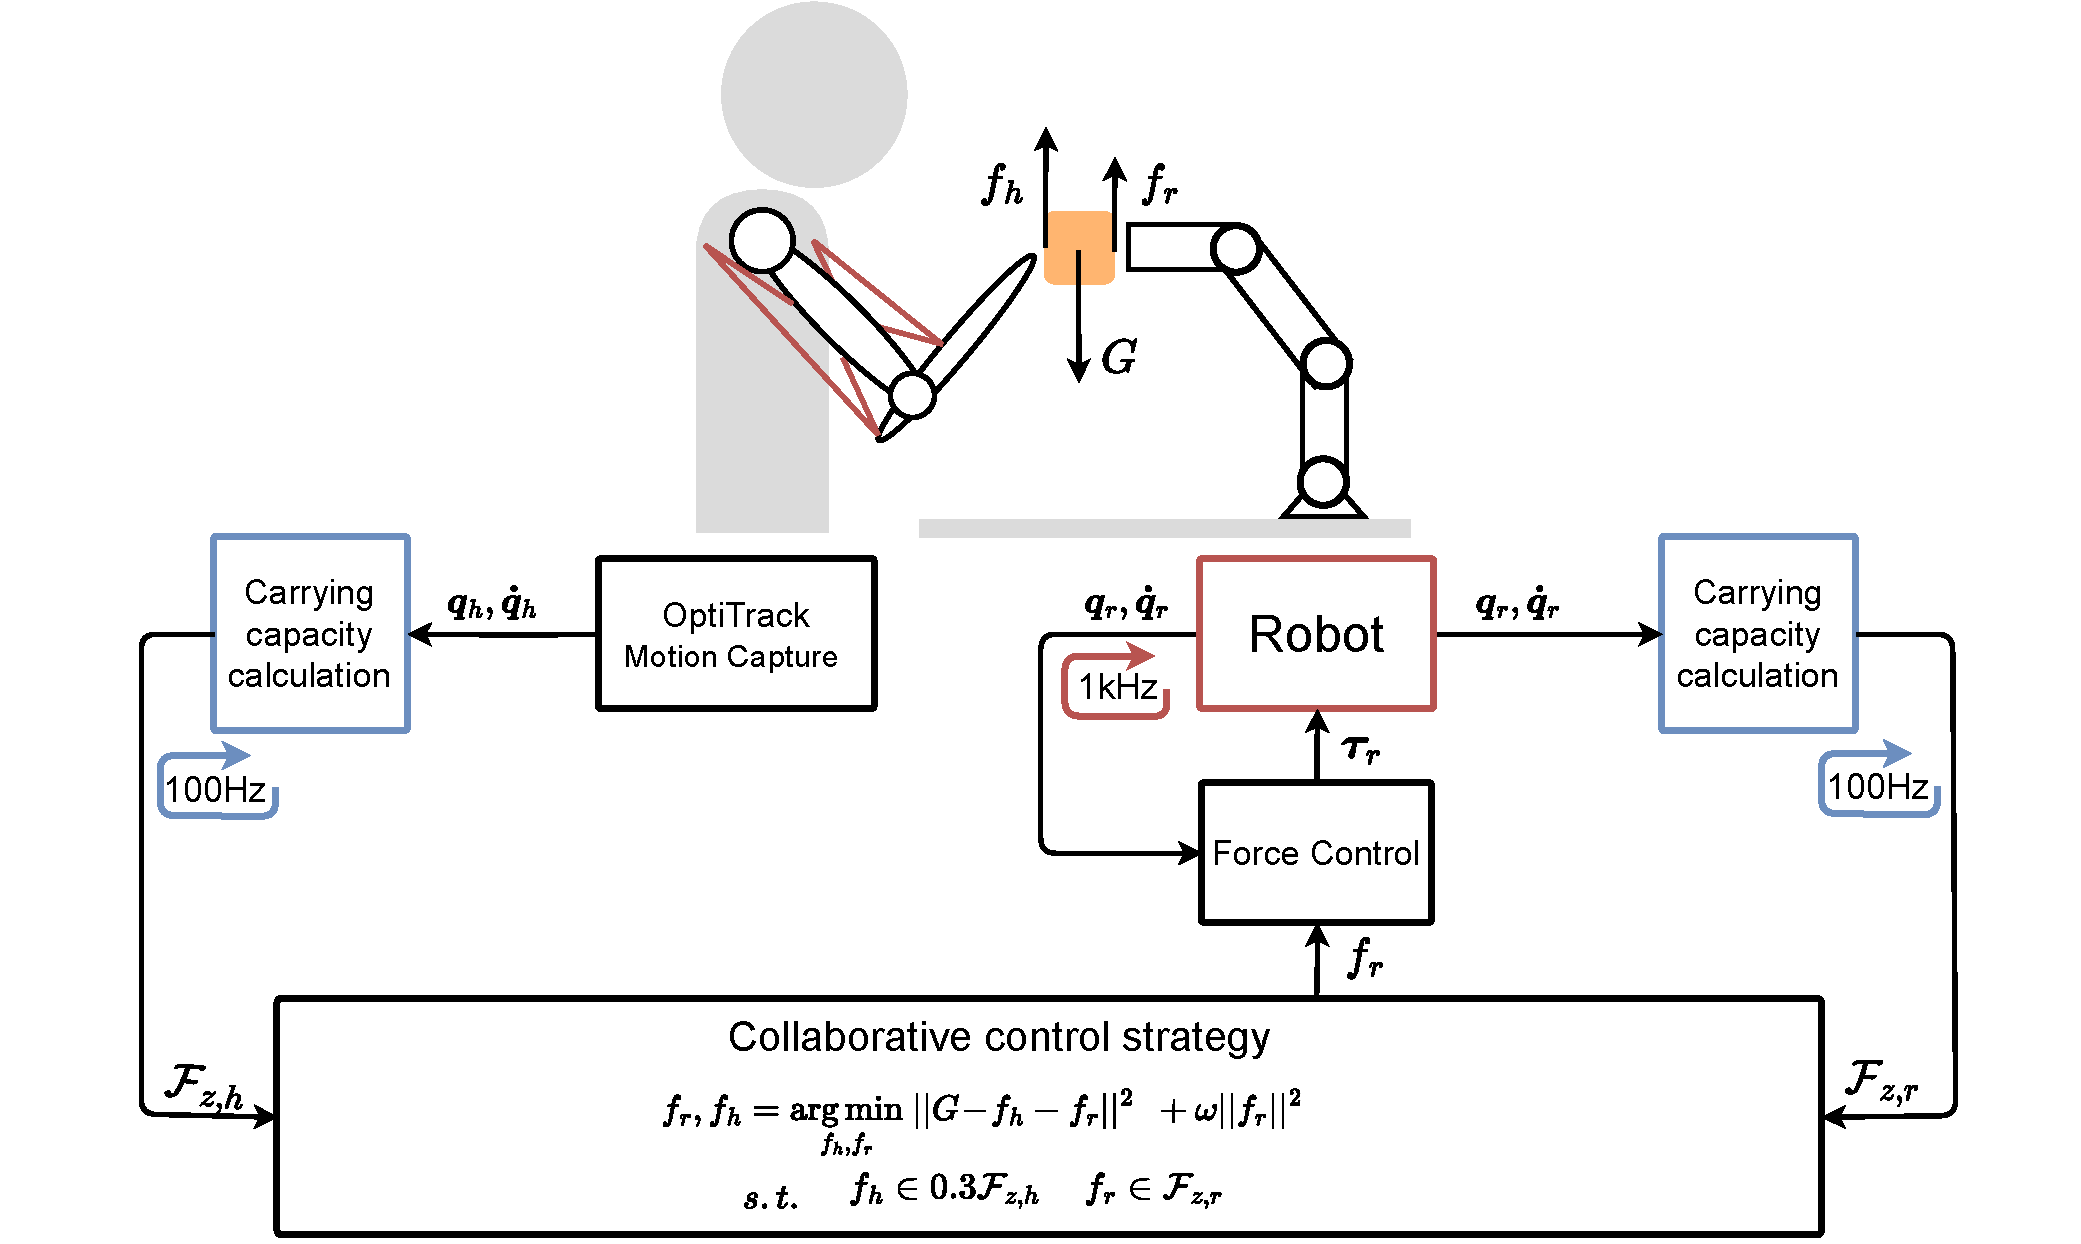
\includegraphics[width=\linewidth]{Papers/images/schema_human_robot.pdf}
    \caption{Block diagram showing the implemented robot control scheme. The robot's low-level force control loop runs at 1kHz, while the carrying capacity calculation of both robot and the operator, as well as the collaborative control strategy, are evaluated at the frequency of 100Hz. Human's posture is obtained using the motion capture system OptiTrack.}
    \label{fig:schema_human_robot_control}
\end{figure}

In each control cycle human's $\mathcal{F}_{z,h}$ and robot's $\mathcal{F}_{z,r}$ carrying capacities are calculated. These values are then used for the resolution of the optimisation problem (\ref{eq:qp_human_robot}). Once the robot's optimal vertical force $f_{r}$ is obtained, the joint torques $\bm{\tau}_{r}$ achieving this force are calculated using the expression
$$
\bm{\tau}_r = J_{z,r}^T(\bm{q}_r) f_r + \bm{\tau}_{b,r}(\bm{q}_r,\dot{\bm{q}}_r)
$$
where $\{\bm{q}_r,\dot{\bm{q}}_r\}\in \mathbb{R}^{n_r}$ is the robot's $n_r$ dimensional state, $J_r\in\mathbb{R}^{\times n_r}$ is the end-effector Jacobian with 1 line and $n_r$ columns, $\bm{\tau}_{b,r} \in\mathbb{R}^{n_r}$ is robot's torque vector corresponding to the effects of the gravity and the robot's motion and $\bm{\tau}_r \in\mathbb{R}^{n_r}$ are the joint torques sent to the robot's low-level joint control. 

The human's force $f_h$, calculated by the proposed control strategy, corresponds to the force the operator should apply in order for the object to stay static in the space. As the weight compensation is both operator's and robot's task, the operator will naturally tend to apply the force $f_h$. 
Therefore, the proposed control strategy indirectly closes the loop with the human operator through the forces applied on the object.

Both robot's and human's carrying capacity calculation algorithms, as well as the robot control strategy described in \Cref{sec:collab_robot_control_human_robot}, are implemented in Python and run in real-time with the update frequency of 100Hz. The low-level robot control is implemented in C++, using the open-source library \codet{pinocchio}~\cite{pinocchio2021}, and run in real-time at the frequency of 1kHz. All the software components are integrated using the \gls{ros}~\cite{ros} and run on a computer equipped with a 1.90GHz Intel i7-8650U processor. 
\Cref{fig:schema_human_robot_control} shows the schematic block diagram of the implemented collaborative robot control strategy. 

\subsection{Experimental validation}
\label{sec:human_robot_experiment}

\begin{figure}[!h]
    \centering
    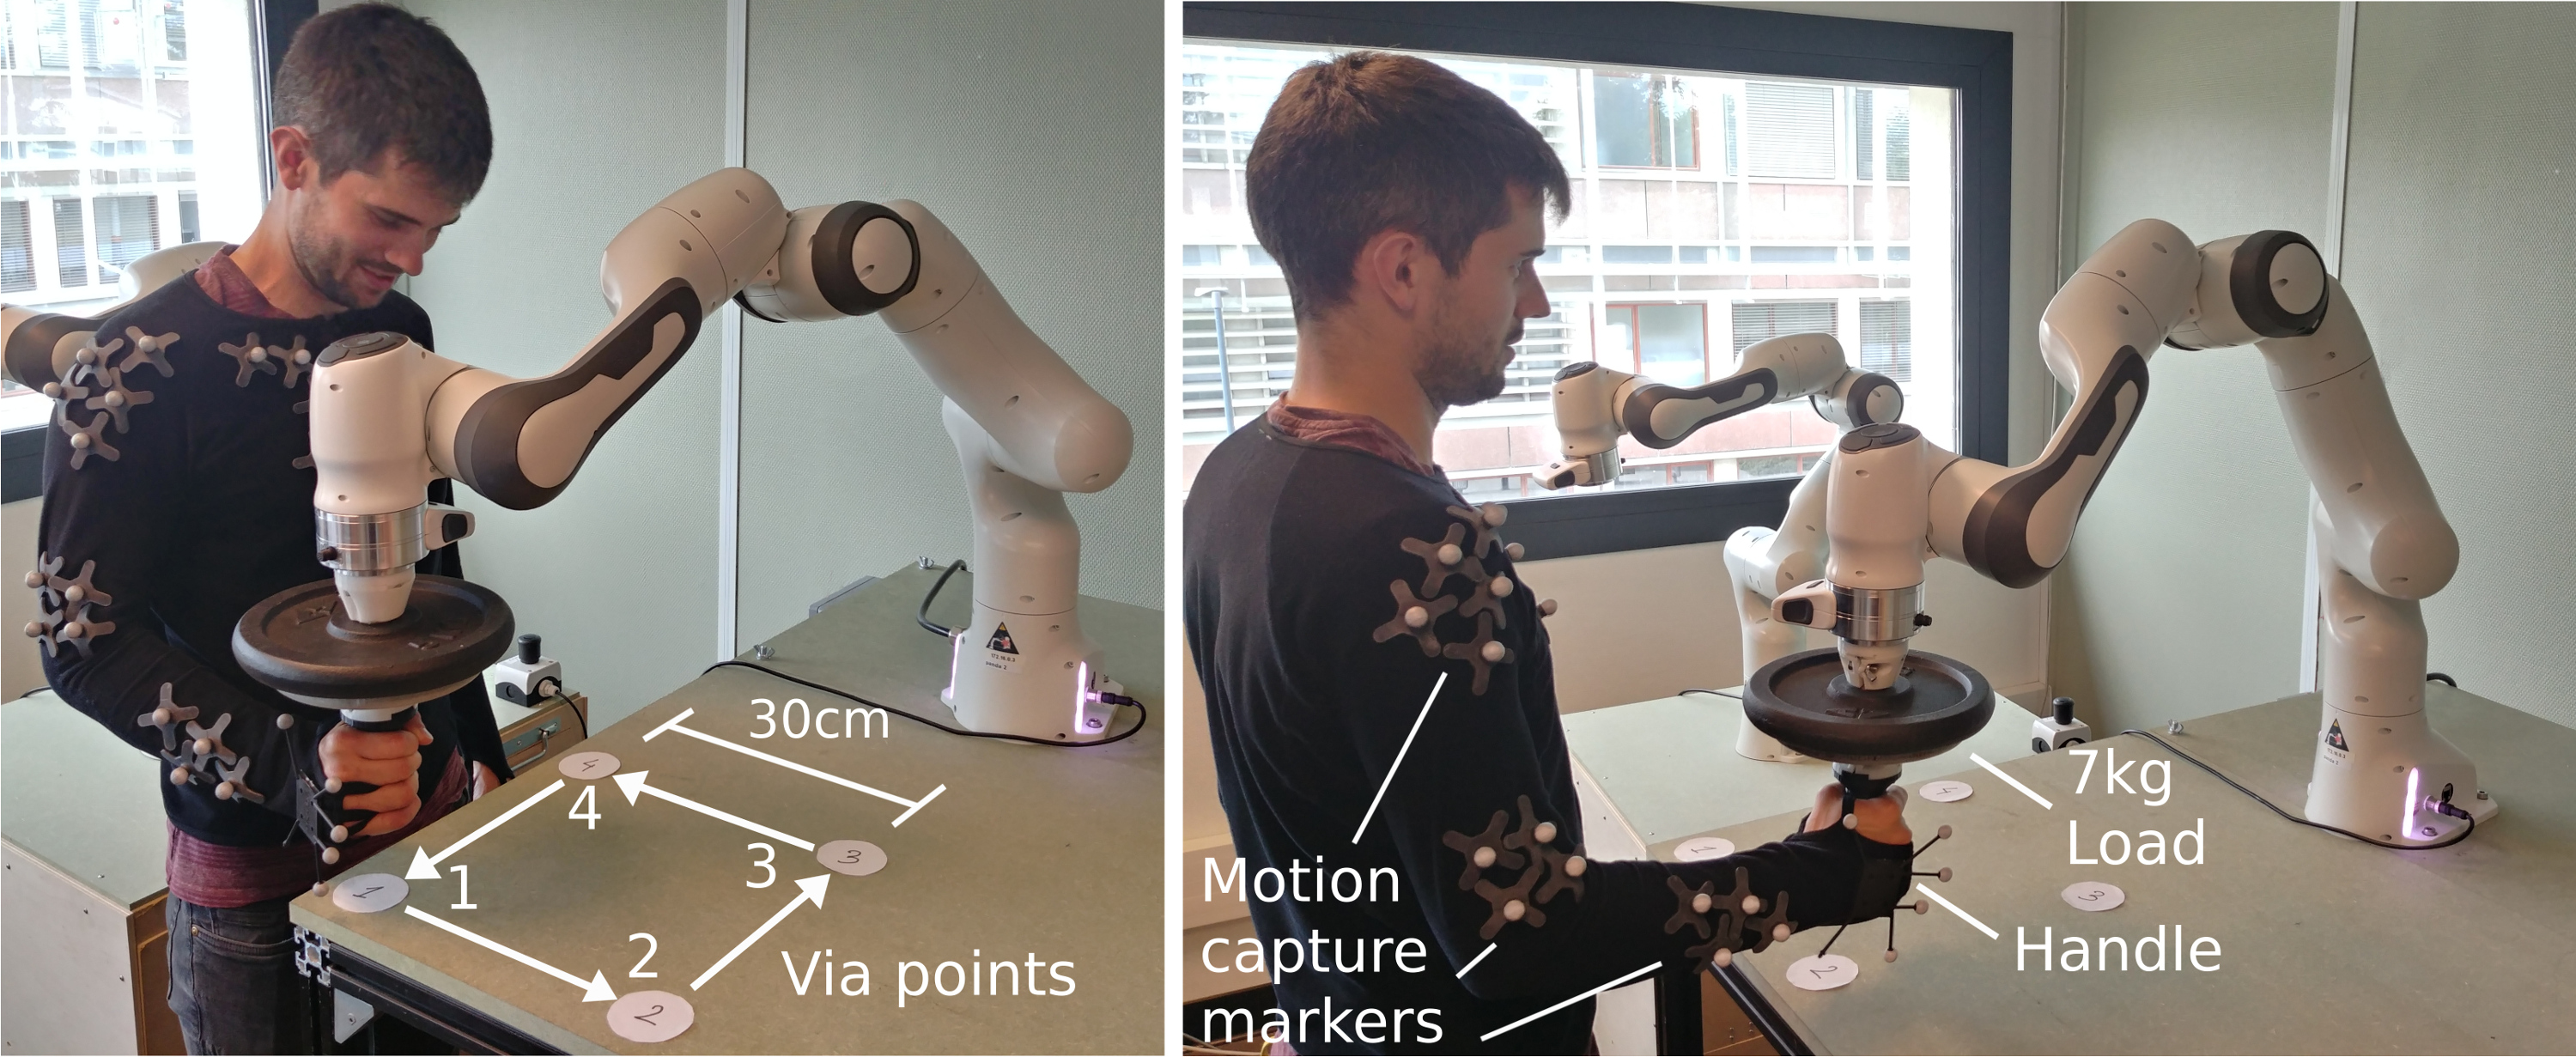
\includegraphics[width=\linewidth]{Papers/images/both_pose_explanation.jpg}
    \caption{{These figures show the experimental setup. The robot end-effector is fixed to the carried object and the human operator is holding the object by the handle. The motion capture system is used to acquire the pose of the human arm. The via-points are visually indicated to the human operator with numbered stickers on the table placed at the corners of a 30 cm square. The images shows the experiment 1 (left) and the experiment 2 (rigth).}}
    \label{fig:experiment2}
\end{figure}

\qrimg{qrcodes/icra2022.png}{https://youtu.be/wg4E62AkNnM}{Video}
In this experiment, the human operator performs a task by {visually} navigating the object through the common workspace, passing through {the set of} 4 via-points. The object is fixed in the end-effector of the robot as well as at the hand of the human operator using a handle. \Cref{fig:experiment2} shows the experimental setup indicating the structure of the collaborative workstation, the placement of the via-points and the handle. 

The experiment is repeated two times, for two different operator positions, equally distant from the via-points, but rotated by 90° in space. These operator positions are indicated on \Cref{fig:experiment2} as well. Furthermore, in each of the two experiments, the operator performs 10 cycles through the via-points. The experiment is illustrated in the accompanying video\footnote{Video: \url{https://youtu.be/wg4E62AkNnM}}.



\begin{wrapfigure}{r}{0.4\linewidth}
\vspace{-0.5cm}
    \centering
    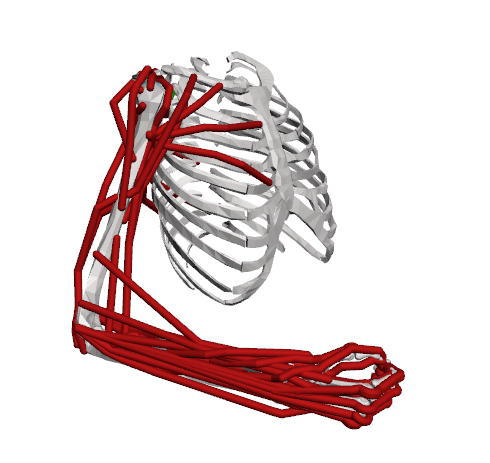
\includegraphics[width=\linewidth]{Papers/images/model_50m7dof.png}
    \caption{Human right arm musculoskeletal model MOBL-ARMS \cite{saul2015benchmarking}, with 50 muscles and 7 joints. Visualised using OpenSim software \cite{opensim}.  }
    \label{fig:model_musc}
\end{wrapfigure}
The musculoskeletal model used in this experiment is the MOBL-ARMS model \cite{saul2015benchmarking} of the human upper limb (right arm), developed by \citet{holzbaur2005model}. A relatively detailed model consisting in 50 muscles ($d=50$) and 7 degrees of freedom ($n=7$). The visualisation of this model, using the biomechanics software Opensim \cite{opensim}, is shown on \Cref{fig:model_musc}.
The operator's arm configuration is inferred in real-time using an OptiTrack~\cite{optitrack} motion capture system. The musculoskeletal model is obtained using the efficient biomechanics library \codet{biorbd} \cite{Michaud2021}. 

The human subject (male, 182 cm, 80 kg) and the MOBL-ARMS model belong to the same 50th percentile anthropomorphic group \cite{gordon1989anthropometric} so no model adaptation is necessary (ex. scaling \cite{correa20112782}).

\Cref{fig:experiment_results} shows the recorded time evolution of robot's and human's carrying capacities and weight carried during the 10 cycles for each of the two experiments. 

The figure shows (top graphs) that the human's carrying capacity is much more variable than the robot's one, peaking around 20kg in the recorded experiments and going as low as 5kg, emphasising the importance of measuring it in real-time, and supporting \Myref{hyp:individual_capacity}. Furthermore, the experiment's show that the human's carrying capacity is in many cases much higher than the robot's capacity, confirming the importance of creating the control strategies able to account for both of their physical abilities. 

\afterpage{
\begin{landscape}
\begin{figure}[!t]
    \centering
    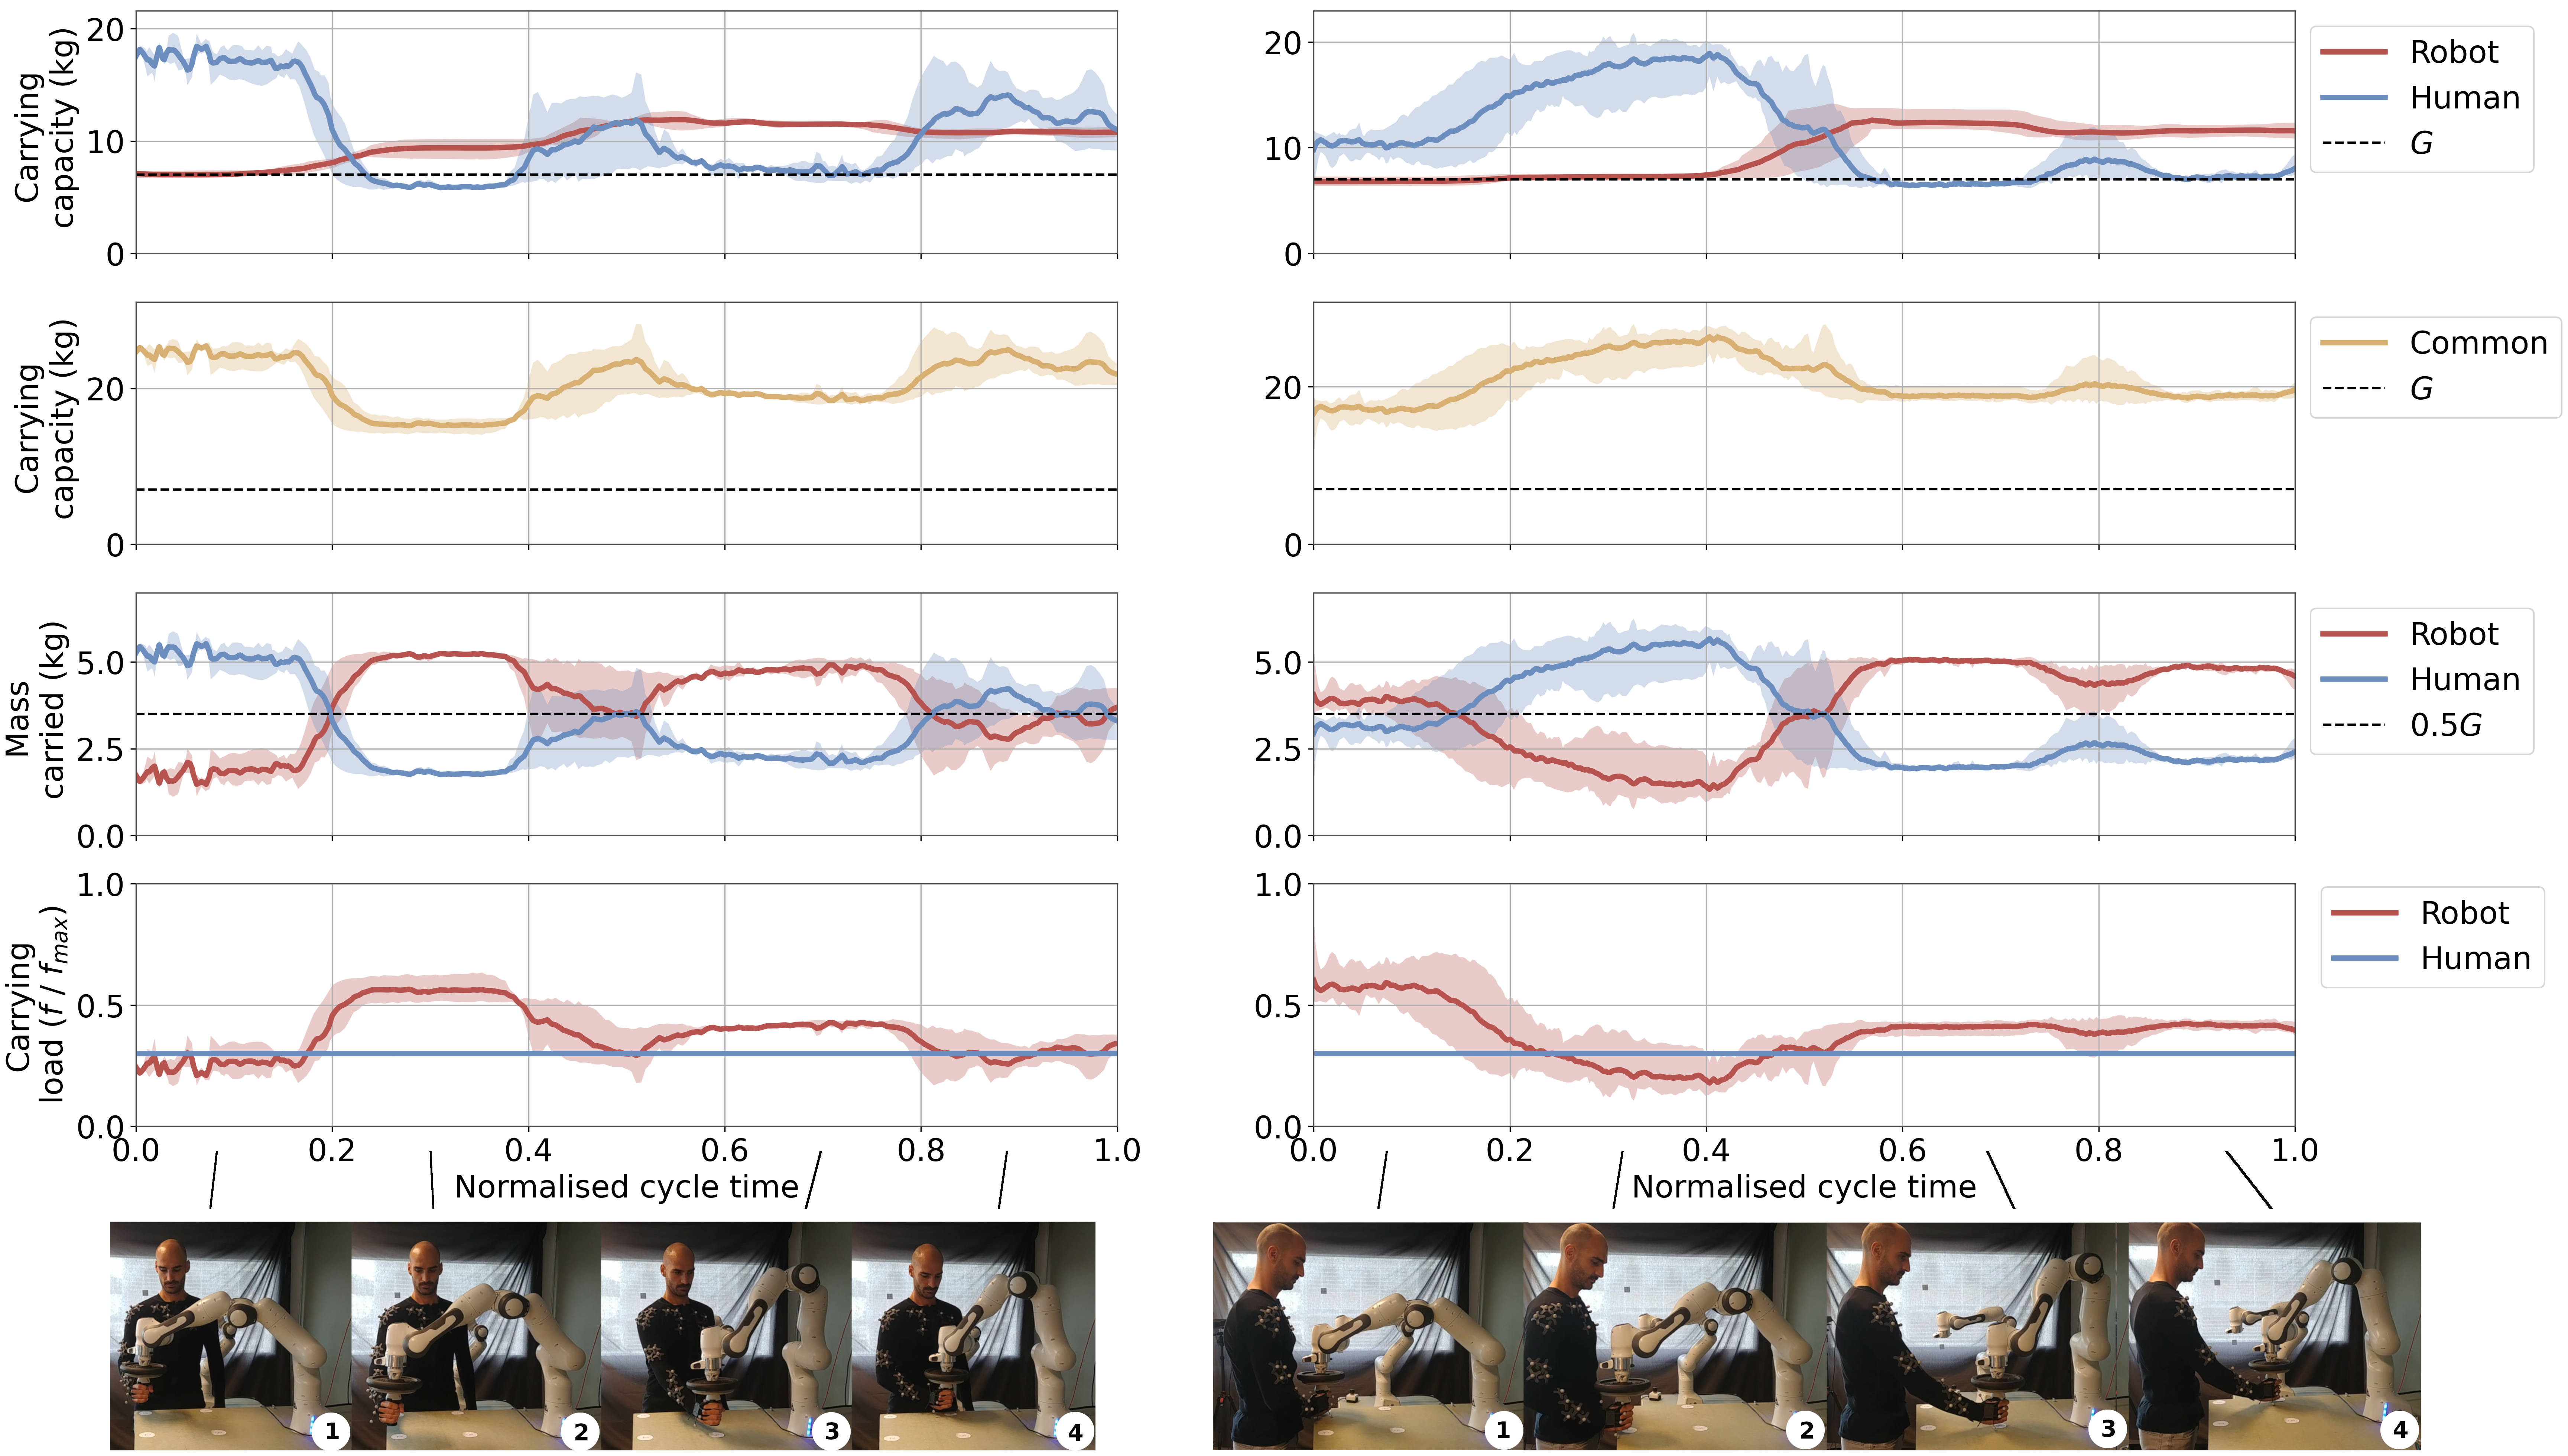
\includegraphics[width=\linewidth]{Papers/images/exp2_new.jpg}
    \caption{This figure shows the evolution of the carrying capacity and weight carried by the operator and the robot over the course of the via-point cycle, for two experiments. The plots show mean values and the variances of the curves calculated over 10 successive cycles. The graph regions belonging to the different via-points are separated by vertical lines.  All the values are expressed in kilograms for easier readability.}
    \label{fig:experiment_results}
\end{figure}
\end{landscape}
}

The second line of graphs on \Cref{fig:experiment_results} shows the time evolution of the sum of their carrying capacities, their common carrying capacity as one system. The graphs show that even though both the robot and the human, in multiple instances during the experiment runs, had carrying capacity lower than the object's weight $G$, their joint carrying capacity exceeds the object's weight during the whole time of the experiment. Therefore, the proposed method demonstrates the feasibility of using physical ability aware control strategies to improve the performance of the physical collaboration. This confirms \Myref{hyp:common_capacity} by showing that, even though, neither the operator or the robot would have been able to carry the object on their own, by collaborating, they were able to execute this task.

It is worth noting that the objective of this experiment is to demonstrate the feasibility rather than guarantee universal applicability. In more general situations, there could be scenarios where the collective carrying capacity of the human and the robot is insufficient to support the object's weight ($f_{h,max}+f_{r,max} <G$). In such cases, the introduced control strategy prioritises ensuring that both actors capacities are not exceeded rather than the complete compensation for the object's weight.

The third line of graphs shows the time evolution of the weight carried by the robot and the human, while the bottom graphs on \Cref{fig:experiment_results}, show the relative load of the robot $l_r$ and the human $l_h$ calculated as
$$
l_h = \frac{f_h}{f_{h,max}}, \qquad\qquad l_r = \frac{f_r}{f_{r,max}}
$$

The graphs confirm that the proposed control strategy maintained the human's relative load at 30\% ($l_h=0.3$) of its capacity as proposed by the \gls{aan} strategy, while the robot's relative load $l_r$ depended on the human capacity. As the human's carrying capacity decreased robot's load $l_r$ increased, and \textit{vice-versa}. By having the real-time knowledge about the operator's carrying capacity, the robot was able to adapt its assistance level to maintain human's load constant, despite substantial changes in the operator's capacity profile and despite his changing placement placement with respect to the task, supporting the \Myref{hyp:safety}.

% In summary, the experimental validation, presented in this section, demonstrates the benefits of integrating accurate real-time information about both the human operator's and the robot's physical abilities within the robot control strategy, in the context of human-robot physical collaboration.

% The proposed robot control strategy exploits both robot's and human's physical abilities, while guaranteeing that neither of their abilities is surpassed. As demonstrated in the experiments, even though their individual abilities are not suitable for executing this task on their own, by collaborating the task become feasible, as their combined abilities (as a single system) are higher than the requirements of the task. In addition to efficiently combining both operator's and robot's physical abilities, the proposed control strategy was able to further ensure safety and operator's engagement in the task, by modulating the weight carried by the human operator in accordance with the proposed \gls{aan} strategy. 

% Finally, the proposed strategy relies entirely on the real-time information about the carrying capacities, enabling very flexible collaborative behaviours, where the robot is able to adapt to any trajectory chosen by the operator as well as to the change in his placement in space. 

\section{Discussion and perspectives}
\label{sec:discussion_perspectives_carrying}
This chapter argues for the use of accurate real-time information about human's and robot's physical abilities for creating collaborative robot control strategies. To demonstrate this concept, the chapter proposes two proof-of-concept experimental scenarios in the context of human-robot physical collaboration. 

As discussed in \Cref{ch:robot_robot_carrying}, the dual robot collaborative carrying experiment shows that the proposed strategy enables to fully exploit the robots' changing physical abilities in real-time. Additionally, the strategy enables ensuring that their safety is not compromised, even though the wight carried by the robots (12kg) is two times higher than their rated payload (2$\times$3kg). Therefore, such real-time capacity-aware control strategies have the potential to enable leveraging the true physical abilities of robots more optimally and even potentially help make a step towards more minimal robot design.

\Cref{ch:human_robot_carrying} showcased the human-robot collaborative carrying experiment. For this scenario a new human-centred robot control strategy is proposed, leveraging the information about both of their physical abilities in real-time. The experiment shows that the strategy successfully distributes weight between the human and the robot, making sure that their abilities are not surpassed, despite their substantial changes happening in real-time. At the same time, the strategy ensures the operator's safety by maintaining the operator's relative load constant (at 30\% of its capacity), inspired by the \gls{aan} paradigm \cite{carmichael2013admittance}.

As the main focus of the experiment is to demonstrate the feasibility of the concept of capacity-aware collaborative robot control, it is important to note that the experiment is conducted with a single participant.
Even though the benefits of similar \gls{aan} strategies have been experimentally confirmed in the rehabilitation literature \cite{Carmichael2013Experimental, petric2019assistive}, their application in the collaborative scenarios is not well studied. Therefore, in order to go a step further and evaluate the utility of such human-centred strategies in more practical applications (and their parameters), a more extensive user study would be required. 

Furthermore, the carrying task, used in the experiments, is relatively simple and essentially one dimensional. However the proposed capacity-aware approaches are not limited to such simple use-cases. \Cref{sec:advanced_collaboraiton_discussion} discusses the perspectives of these approaches to be used in more complex human-robot physical collaboration scenarios. 
Moreover, the experiments demonstrated that the computational efficiency of the ICHM algorithm allows for using a relatively detailed human musculoskeletal model of operators to evaluate their physical abilities in real-time. \Cref{sec:human_robot_prospective} discusses the benefits and limitations of using such detailed human models in the context of human-robot collaboration.


\subsection{Perspective: Extension to more flexible assistive strategies}
\label{sec:advanced_collaboraiton_discussion}

The proposed human-robot collaborative carrying experiment, as discussed in \Cref{sec:human_robot_experiment}, has two main limitations. Firstly, it only accounts for forces in the vertical ($z$-axis) direction, limiting the task to one-dimensional ($m=1$) space. This simplification reduces computational complexity but does not exploit full polytope geometry of the human's and robot's physical abilities. Secondly, the wrenches ($\bm{f}_h$) applied by the human operator are not measured in the experiment, simplifying the scenario by assuming all operator forces are in the $z$-axis direction. However, in the absence of wrench $\bm{f}_r$ measurements, the operator receives no assistance for forces orthogonal to the $z$-axis. 

One of the promising approaches able to address these limitations is proposed by \citet{petric2019assistive}.
The authors proposed an assistive strategy based on human's force ellipsoids, where the robot's task consists in making the operator's force capacity isotropic (equal in all the directions in space). The forces applied by the operator are measured in real-time and amplified by the robot. The amplification factor is determined with respect to the operator's force capacity in the direction of the applied force. The author's show that such strategy does not restrict the operator's movements while significantly reducing the effort. However, their work is based on force ellipsoids which are a coarse under-approximation of the true operator's force capacity. Moreover, their approach is created around a very specific planar exoskeleton setup in the rehabilitation context. Therefore, this section discusses an extension of this approach to the polytope representation of physical abilities and to more flexible collaboration scenarios. 

Such human-centered assistive robot control strategy could enable providing the operator with adapted assistance in any spatial direction, by leveraging the real-time measurement of the operator's wrenches $\bm{f}_h$. Moreover, the method could allow for exploiting the full polytope geometry of human's and robot's wrench polytopes ($\mathcal{P}_{f,h}$ and $\mathcal{P}_{f,r}$). Finally, such method could allow to shape the operator's wrench capacity given a desired polytope $\mathcal{P}_{f,d}$, opening doors for more flexible collaboration behaviours.

\begin{figure}[!h]
    \centering
    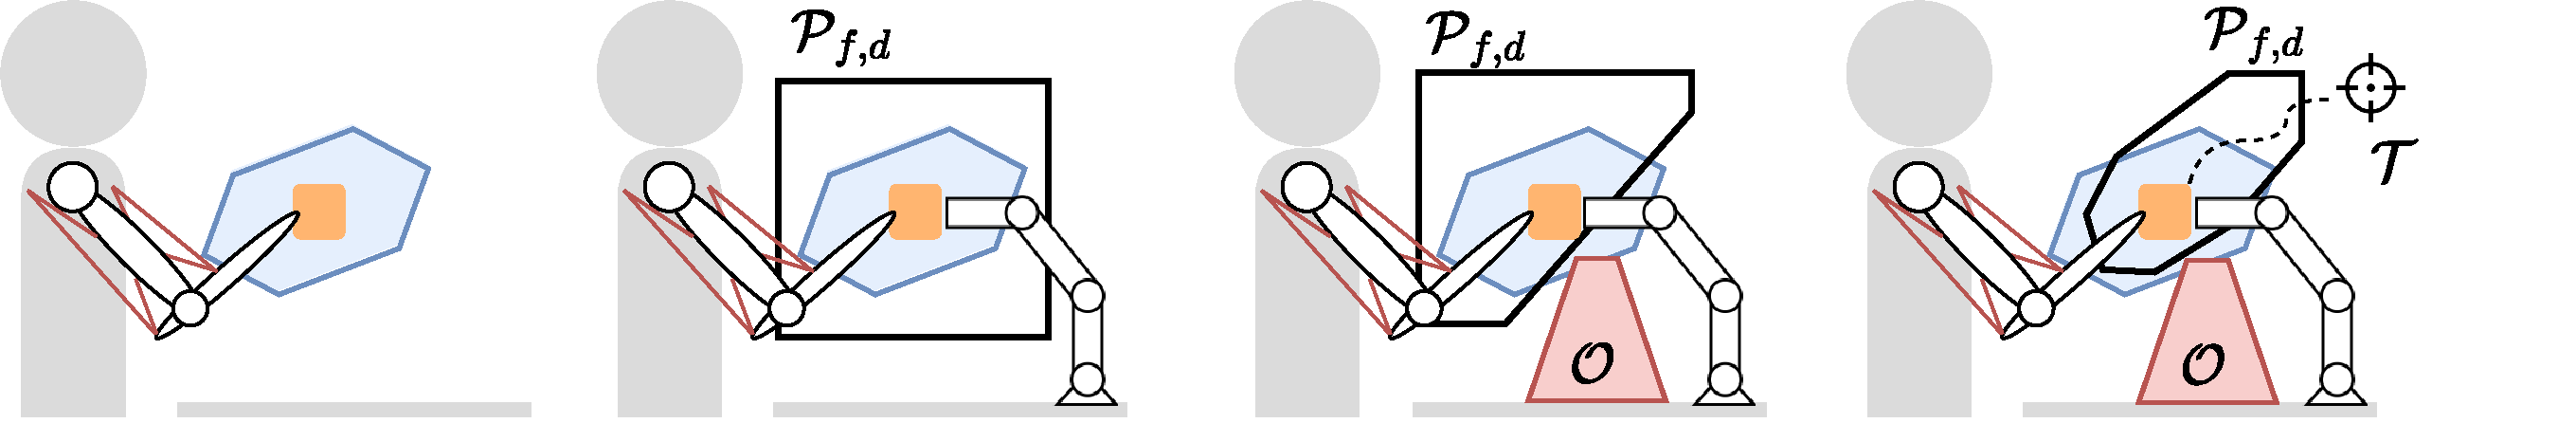
\includegraphics[width=\linewidth]{Papers/lichie/modulatio_all.pdf}
    \caption{This figure illustrates the proposed assistive control strategy based on the desired polytope $\mathcal{P}_{f,d}$ modulation. The first figure on the left shows the human's wrench polytope $\mathcal{P}_{f,h}$ with no robotic assistance. The second figure shows the case where the robotic assistance leads to the isotropic rectangle shape of the desired polytope $\mathcal{P}_{d,f}$. The third figure shows the scenario where the desired polytope is modulated in order to prevent collision with the obstacles $\mathcal{O}$. The last figure shows the scenario where the desired polytope $\mathcal{P}_{f,d}$ shape takes in account the obstacles and guides the operator in the executing the task $\mathcal{T}$.}
    \label{fig:desired_modulaiton}
\end{figure}

By setting an appropriate shape of the desired polytope $\mathcal{P}_{f,d}$, different collaborative behaviours can be obtained. 
For example, if no information about the task and the environment is available, then the shape $\mathcal{P}_{f,d}$ can be set to a $m$-dimensional hypercube. In this scenario, the robot's assistance makes the operator's force capacity isotropic (equal in all the directions of the space).
On the other hand, if the information about the obstacles in the environment is available, the shape of the desired polytope $\mathcal{P}_{f,d}$ can be reduced in the directions of obstacles, preventing the operator to get in contact with them.
Finally, if the operator's task requires executing a trajectory, known in advance, the shape of the desired polytope $\mathcal{P}_{f,d}$ can be chosen to guide the operator toward the successful task execution.
\Cref{fig:desired_modulaiton} illustrates the discussed  behaviours through of the desired polytope $\mathcal{P}_{f,d}$ modulation.

\subsubsection*{Implementing the adaptive force amplification approach}

\begin{wrapfigure}[13]{r}{0.30\linewidth}
\vspace{-0.5cm}
    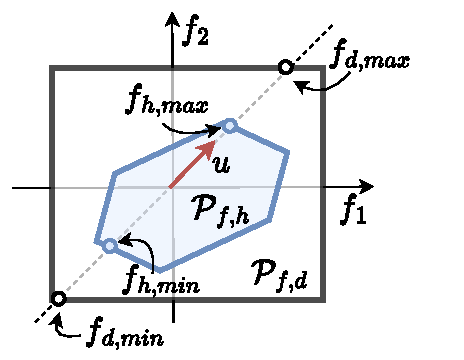
\includegraphics[trim=0.6cm 0cm 0.9cm 0.2cm,clip=true,width=\linewidth]{Papers/lichie/max_desired.pdf}
    \caption{Finding the maximal ranges of human's and desired wrench capacity in direction $\bm{u}$. }
    \label{fig:max_desired}
\end{wrapfigure}
For a given operator wrench $\bm{f}_h$, characterised by magnitude $f_h$ and direction vector $\bm{u}$, both operator and robot force capacity intervals can be defined: $f_h \in [f_{h,min}, ~f_{h,max}]$ and $f_r \in [f_{r,min}, ~f_{r,max}]$, as detailed in \Cref{sec:human_carrying_capacity} and \Cref{sec:robot_carrying_capacity}. Using the same vector $\bm{u}$, the maximum desired range $[f_{d,min}, ~f_{d,max}]$ within the polytope $\mathcal{P}_{f,d}$ can be determined.
\Cref{fig:max_desired} illustrates the geometrical representation of these ranges.

The proposed assistive robot control strategy consists in amplifying the operator's wrench as follows
\begin{equation}
\bm{f}_r = \underbrace{\alpha f_h}_{f_r}\bm{u}
\label{eq:force_amp_perspective}
\end{equation}
Here, $\alpha$ represents a scalar amplification factor and $f_r$ is the magnitude of the robot's wrench applied in the direction $\bm{u}$. 
The final force applied jointly by the robot and the human is then
\begin{equation}
f_h + f_r = (1+\alpha)f_h
\end{equation}
In order to amplify the operator's force capacity $f_{h,max}$ in the direction $\bm{u}$, and match the desired capacity $f_{d,max}$, the factor $\alpha$ can be determined using the ratio
\begin{equation}
\frac{f_{h}}{f_{h,max}} = \frac{(1 + \alpha) f_h}{f_{d,max}}
\end{equation}
The final expression for the amplification factor $\alpha$ becomes
\begin{equation}
\alpha = \frac{f_{d,max}}{f_{h,max}}-1
\label{eq:alpha_perspective}
\end{equation}

To calculate the amplification factor $\alpha$ (\ref{eq:alpha_perspective}), while at the same time ensuring that the robot's wrench capacity is not exceeded, a \gls{qp} can be formulated
\begin{equation}
    \begin{split}
        \alpha =\underset{\alpha}{\arg\min} &~\Big|\Big|\alpha- \frac{f_{d,max}}{f_{h,max}}+1\Big|\Big|^2\\
        s.t.& \quad f_r  = \alpha f_h\\
        & \quad f_r \in[f_{r,min}, ~f_{r,max}]\\
    \end{split}
    \label{eq:qp_human_robot_perspective}
\end{equation}

For any human wrench ($\bm{f}_h=f_h\bm{u}$), the assistive robot control strategy (\ref{eq:qp_human_robot_perspective}) allows to calculate the optimal force amplification $\alpha$, shaping the operator's wrench capacity $\mathcal{P}_{f,h}$ into the desired shape $\mathcal{P}_{f,d}$, while respecting the robot's wrench capacity $\mathcal{P}_{f,r}$. 

\subsubsection*{A parallel with the impedance control}
Consider that the operator and the robot jointly manipulate an object with a mass $m$. The wrenches they apply onto the object are combined and produce its motion in space
\begin{equation}
    \bm{f}_h + \bm{f}_r = (1+\alpha)\bm{f}_h = m \ddot{\bm{x}}
\end{equation}
where $\ddot{\bm{x}}$ is the object's \gls{cs} acceleration (including gravity) and $\alpha$ is the amplification factor described in the previous section. This equation can be rearranged in a form
\begin{equation}
    \bm{f}_h = \frac{m}{1+\alpha} \ddot{\bm{x}}
\end{equation}
permitting to see the proposed assistive approach as a special case of the impedance control, allowing to modulate the perceived mass $m$ of the object to the operator. 
This approach could enable the intuitive modulation of the perceived mass of the object through the desired polytope $\mathcal{P}_{f,d}$, providing the operators with physical feedback about the task and their environment. Additionally, the object's mass can be modulated to account for the changing physical abilities of the operator $\mathcal{P}_{f,h}$ and the robot $\mathcal{P}_{f,r}$. 

However, in the context of this thesis, the development of this approach stayed in the conceptual stage, leaving it as a potential avenue for future research and exploration.


\subsection{Perspective: On using detailed musculoskeletal models}
\label{sec:human_robot_prospective}

The ICHM algorithm, proposed in \Cref{ch:algorihtm_ichm}, presents a new and efficient way of evaluating different polytopes of physical abilities based on human's musculoskeletal models. This algorithm opens many possibilities for wider use of human physical ability polytopes in the area of the human-robot collaboration, by both reducing the computation time and enabling the use of more complete human models, better describing human subjects \cite{sohn2019effects}. 

The algorithm's real-time ability may enable higher degree of human-centred robot control, where the operators' accurate real-time capacity, based on the detailed musculoskeletal models, could be used not only to enforce safety and improve engagement, but to provide the operator-specific assistance profiles. Such detailed musculoskeletal models could help preventing the development of the work related injuries, by ensuring that the operator's load well suited to its abilities as well as by including the information about his fatigue level \cite{Bolghanabadi2014fatigue} or his specific pathology. Furthermore, in more distant future, such human-centred approaches could be used to create scenarios in which the operator's load would not be adapted just to its current abilities, but modulated in a way to increase his abilities over time or potentially even enable the rehabilitation in the factory context. 

However, even though the ICHM algorithm, and the potential collaborative robot control strategies using it, are independent of any musculoskeletal model, their accuracy relies entirely on the model's real-time representation of the operator. Therefore, for practical implementations, the key challenges are two-fold: evaluating human posture in the real-time, precise enough and in a minimally intrusive way, as well as performing the individual scaling and calibration of the used musculoskeletal models for a given operator \cite{correa20112782}.

In their recent work, \citet{laisne2023Genetic} have proposed a new promising method for calibrating the musculoskeletal models of human subjects, based in part on the works conducted in this thesis, particularly on the ICHM algorithm. The method consists in measuring the human subject's force capacity polytope in the laboratory setup and finding the optimal parameters of the musculoskeletal models to minimise the error between the recorded and simulated polytope. The method is based on the optimisation using Genetic algorithms and is applicable to relatively detailed musculoskeletal models, such as the model with 50 muscles and 7 joints developed by \citet{holzbaur2005model}.

Such techniques have a great potential to enable using detailed and well adapted models of the human operators and, in combination with the efficient tools for their analysis, enable high degree of personalised assistance to the operators, further improving their well-being and safety.


\section{Conclusion}

This chapter showcases the potential of employing polytope representations of robots' and humans' physical abilities to develop collaborative robot control strategies capable of adaptation to their changing abilities online. The chapter demonstrates that real-time calculation of these polytopes provides promising tools for creating flexible robot control strategies for different physical collaborating scenarios. Allowing the robot to adapt not just to the requirements of the task and its own abilities, but also to the changing abilities of the operators and their safety.

The chapter attempts to demonstrate three concepts, stating the potential impact of using real-time information about robot's and human's physical abilities for creating the adaptive robot control in collaborative scenarios. \Myref{hyp:individual_capacity} states that this real-time information can be exploited to better use each of the actors individual abilities. 
\Myref{hyp:common_capacity} states that such real-time information can be used to better distribute the task load and allow them to collaboratively perform the task they would have been unable to do on their own. Finally, \Myref{hyp:safety} states that the human's real-time capacity information can be used to improve his safety and well-being while executing the task.

To support these concepts, the chapter brings two example collaborative scenarios, based on a common industrial task of collaborative carrying of a heavy object. The scenarios studied are: dual robotic arm collaborative carrying and human-robot collaborative carrying. 

In the dual robot arm experiment two Franka Emika Panda robots carry an object with a mass of 12 kg through the common workspace, even though their rated payload, given by the manufacturer, is 3kg. 
Robots' carrying capacity is calculated in real-time using the algorithm VEPOLI$^2$, proposed in \Cref{sec:algorithm_vea}. This real-time information is then used to create the collaborative robot control strategy that adapts to their changing capacities in real-time.

The experiment shows that by calculating robots' carrying capacity in real-time, each one of the robots is able to surpass their rated abilities without compromising their safety, demonstrating \Myref{hyp:individual_capacity}.
Furthermore, by using the real-time information about the carrying capacity of both robots, the proposed control distributes the weight of the object to the robots with respect to their changing physical abilities. As a result, the experiment shows that the two robots are able to compensate for the 12kg weight during the whole time of the experiment, even though neither of the robots would have been able to carry half of the object's weight on their own, demonstrating \Myref{hyp:common_capacity}. This experiment has been published as a part of the scientific article \citet{skuric2021robot}.

In the second experiment, human operator and a Franka Emika Panda robot jointly carry 7kg object. Human's and robot's carrying capacity are calculated in real-time and used to create the collaborative robot control strategy adapting to their real-time changes.
In order to determine the human's carrying capacity, a relatively detailed musculoskeletal model of the human right arm is used, with 50 muscles and 7 joints, developed by \citet{holzbaur2005model}. Then, the newly developed algorithm ICHM, described in \Cref{ch:algorihtm_ichm}, is used to do the real-time calculations.

The experiment reveals that human carrying capacity exhibits greater variability compared to that of the robot. Interestingly, in several instances, the human demonstrated a higher carrying capacity than the robot. 
By having real-time information about the carrying capacities of both the human and the robot, the proposed control strategy effectively distributes the weight between them, while making sure that their both physical abilities are not exceeded. Even though neither of them would have been able to carry the object on their own, the proposed control strategy enables them to successfully carry out the task when collaborating physically, once again demonstrating \Myref{hyp:common_capacity}. 

Moreover, in addition to to making sure that human's physical ability is not surpassed during the task executions, to further demonstrate \Myref{hyp:safety}, an additional task was incorporated into the collaborative robot control strategy aiming to improve the operator's safety and his engagement in the task. This task consisted in maintaining a constant relative load for the operator throughout the experiment, corresponding to 30\% of its carrying capacity. This concept was inspired by the \gls{aan} strategy as described in \citet{carmichael2013admittance}, commonly used in rehabilitation and assistance robotics. The human-robot collaborative carrying experiment has been published as a part of the scientific article \citet{Skuric2022human}.

In conclusion, this chapter advocates for creating robot control strategies based on the real-time and accurate information about the changing nature of task related physical abilities of robots and humans, based on polytopes. The chapter shows that such strategies enable employing their individual abilities fully without compromising their safety. Furthermore, when collaborating physically, such strategies enable distributing their task execution load with regard to their changing abilities, allowing them to execute tasks they would not have been able to do individually. Finally, the chapter shows that having the real-time and accurate information about human's physical abilities has a great potential to further improve operator's safety and well-being at the workplace. 


Following two chapters explore the potential use-cases of the real-time physical ability polytope evaluation in different human-robot collaboration scenarios. \Cref{ch:informaiton_polytopes}, explores the possibilities of using polytopes for the real-time visual feedback to the operators. \Cref{ch:topca} proposes a new \gls{cs} trajectory planning strategy exploiting the polytope algebra. 
Finally, \Cref{ch:software} presents a publicly available open-source software Python package \codet{pycapacity}, providing tools for the efficient evaluation of polytope and ellipsoid based physical abilities of humans and robots.

